\documentclass[11pt,a4paper]{article}

\usepackage[margin=1in]{geometry}
\usepackage{amsmath,amssymb}
\usepackage{booktabs}
\usepackage{tabularx}
\usepackage{array}
\usepackage{float}
\usepackage{wrapfig}
\usepackage{graphicx}
\usepackage{listings}
\usepackage{xcolor}
\usepackage{tikz}
\usetikzlibrary{arrows.meta,positioning,shapes.geometric}
\usepackage{hyperref}
\usepackage{cite}
\usepackage[title,titletoc]{appendix}

\hypersetup{
    colorlinks=true,
    linkcolor=blue,
    citecolor=blue,
    urlcolor=blue
}

\lstset{
    basicstyle=\ttfamily\scriptsize,
    keywordstyle=\color{blue}\bfseries,
    commentstyle=\color{gray}\itshape,
    stringstyle=\color{teal},
    breaklines=true,
    frame=single,
    tabsize=2,
    showstringspaces=false,
    captionpos=b,
    numbers=none
}

\title{\textbf{Final Report: L2 TLB Support for Sparse Huge Pages}}
\author{\textbf{CS622 Course Project}}
\date{November 2026}

\begin{document}

\maketitle

\begin{abstract}
Virtual memory address translation overhead represents a performance bottleneck in computing systems, accounting for 10\% to 40\% of execution cycles in data-intensive workloads. This report covers the whole project on L2 TLB architectures in the \texttt{gem5} simulator~\cite{binkert2011gem5}, in two parts.

\textbf{Part I} is our mid-review report. It refactors the L2 TLB into a 128-set, 4-way set-associative array with XOR-7 indexing and evaluates Inclusive, NINE and Exclusive inclusion policies, Sequential and Naive Free Prefetching, CoLT-FA (\textbf{52.19\% L2 miss reduction}), Perforated Pages (\textbf{4.16$\times$ speedup} on clustered versus dispersed fragmentation) and a prototype Hybrid L2 TLB (\textbf{71.22\% L2 miss reduction}), all in syscall-emulation (SE) mode on microbenchmarks.

\textbf{Part II} covers the work after the mid-review. An audit of all designs found problems that only appear under a real operating system: missing L2 invalidation on page unmaps and address-space switches, PCID handling, checkpointing and hard-coded permissions. We fixed six designs (Inclusive, Exclusive, NINE, Agile/NaiveFP, Perforated Pages and CoLT-FA), added a translation oracle and invariant checkers, and found \textbf{no translation error} in any design. We rebuilt CoLT-FA so that it coalesces pages from the hardware page walker, which made it work in full-system mode. In full-system \texttt{gem5} on an Ubuntu 24.04 guest, \textbf{37 of the 43 SPEC CPU2017 benchmarks pass on every design}, and none of the failures is caused by the TLB. On TLB-intensive workloads, CoLT-FA reduces page walks compared with NINE by \textbf{59\% to 64\%} on GAPBS bfs, cc and sssp with 4KB pages. A closer look at Perforated Pages shows that its large gains come from an unrealistic model. The report ends with an appendix describing the submitted artifact and how to evaluate it.
\end{abstract}

\newpage
\tableofcontents
\newpage

\part{Progress up to the Mid-Review}
\label{part:mid}
% =============================================================================
% PART I: PROGRESS UP TO THE MID-REVIEW (original mid-review report content)
% =============================================================================

% -----------------------------------------------------------------------------
\section{Introduction and Problem Formulation}
% -----------------------------------------------------------------------------

\subsection{The Memory Translation Wall}
Operating systems rely on paging to provide hardware isolation, process placement, and memory overcommitment. However, converting a 64-bit Virtual Address (VA) to a Physical Address (PA) under x86-64 long-mode requires traversing a 4-level or 5-level hierarchical page table structure: Page Map Level 4 (PML4), Page Directory Pointer Table (PDPT), Page Directory (PD), and Page Table (PT). Each level requires a memory access. In the worst case, a memory read or write instruction may trigger up to four memory references, inducing latencies of processor clock cycles.

Hardware Translation Lookaside Buffers (TLBs) act as caches for translations. Microarchitectures implement a split two-level TLB hierarchy:
\begin{itemize}
    \item \textbf{Level-1 (L1) TLB}: Split into an Instruction TLB (ITB) and Data TLB (DTB), holding 32 to 64 entries, operating with single-cycle hit latencies.
    \item \textbf{Level-2 (L2) TLB}: Unified, holding 512 to 1536 entries, operating within 7 to 12 clock cycles to intercept L1 misses before initiating hardware page table walks.
\end{itemize}

Despite multi-level caching, a 512-entry L2 TLB configured with 4KB pages covers:
\begin{equation}
    \text{Reach} = 512 \times 4\text{ KB} = 2\text{ MB}
\end{equation}
Workloads, ranging from in-memory databases and graph analytics to graph neural networks and cloud virtualization, manipulate working sets exceeding tens of gigabytes. Under such working sets, TLBs experience thrashing, where Translation Table Walks (TTWs) account for up to 40\% of execution time.

\subsection{Limitations of Existing Solutions}
Three mechanisms attempt to mitigate this translation bottleneck, each with shortcomings:
\begin{enumerate}
    \item \textbf{Superpages (2MB Huge Pages)}: x86 architectures support 2MB superpages by terminating page table traversal at the Page Directory level. While a 2MB page increases TLB reach by $512\times$, operating systems (e.g., Linux Transparent Huge Pages) require 2MB of \textit{physically contiguous, aligned memory}. Over execution, memory becomes fragmented by non-movable pages, slab caches, and device buffers. When fragmentation prevents 2MB contiguous allocation, the operating system fractures the region into 512 4KB pages, forfeiting superpage reach.
    \item \textbf{Hardware TLB Prefetching}: Speculative page prefetchers monitor virtual address strides to load PTEs into the TLB ahead of demand requests. However, unguided prefetchers generate memory bus traffic and pollute cache ways when access strides diverge or become irregular.
    \item \textbf{Hierarchy Policies}: Processor L2 TLBs employ inclusive or non-inclusive replacement policies, duplicating translation tags across L1 and L2 and reducing the aggregate reach of the core's MMU.
\end{enumerate}

\subsection{Project Scope and Research Objectives}
The objective of this ongoing research is to investigate, implement, and evaluate microarchitectural solutions to the translation reach problem using the \texttt{gem5} simulator~\cite{binkert2011gem5}. Specifically, we:
\begin{itemize}
    \item Refactor the flat x86 TLB model in \texttt{gem5} into a 128-set, 4-way set-associative array and characterize the performance trade-offs of Inclusive, NINE, and Exclusive inclusion policies~\cite{baer1988multi} under stress workloads.
    \item Explore translation-level prefetching techniques that exploit cache-line spatial locality, comparing Sequential Prefetching (SP) with Naive Free Prefetching (NaiveFP)~\cite{margaritov2019prefetched}.
    \item Replicate and evaluate the Coalesced Large-Reach TLBs (\textbf{CoLT}, MICRO 2012~\cite{pham2012colt}) architecture, specifically comparing Set-Associative coalescing with a Fully-Associative (CoLT-FA) coalescing buffer.
    \item Replicate and evaluate \textbf{Perforated Pages} (ISCA 2020~\cite{kwon2020perforated}), modeling sparse huge-page descriptors, two-level coarse filtering, latency/energy accounting, and decoupled in-TLB bitmap caching.
    \item Formulate, build, and validate a prototype \textbf{Hybrid L2 TLB} that synthesizes CoLT buffer absorption with fragmented 2MB perforated superpage coverage.
\end{itemize}

% -----------------------------------------------------------------------------
\section{Simulation Framework and Methodology}
% -----------------------------------------------------------------------------

\subsection{The gem5 Simulator Framework}
Architectural modeling was conducted within \texttt{gem5} (version 25.1.0.1)~\cite{binkert2011gem5} targeting the x86-64 instruction set architecture. \texttt{gem5} provides execution-driven, cycle-level timing simulation of processor pipelines, caches, and memory management units.

Simulations were executed in \textbf{Syscall Emulation (SE)} mode. In SE mode, \texttt{gem5} intercepts Linux system calls and emulates memory allocation, process address spaces, and page tables through an internal \texttt{EmulationPageTable} instance. While SE mode abstracts away operating system kernel thread scheduling, it provides cycle-level accuracy for the processor core, MMU request pipeline, cache hierarchy, and page walker state machines.

\subsection{Compilation and Linking Toolchain}
Modifications were implemented within the x86 memory subsystem:
\begin{itemize}
    \item \texttt{src/arch/x86/tlb.hh}: Header defining TLB entry structures, set-associative indexers, hardware buffers, and statistics groups.
    \item \texttt{src/arch/x86/tlb.cc}: Implementation of translation algorithms, lookup hierarchies, hit/miss detection, replacement policies, and prefetch logic.
    \item \texttt{src/arch/x86/pagetable.hh}: Paging structures and page alignment definitions.
\end{itemize}

During builds of \texttt{build/X86/gem5.opt}, the compilation environment encountered virtual memory consumption during the link phase of the binary, triggering host out-of-memory (OOM) swap thrashing. To eliminate this bottleneck, the build system was configured to use the GNU \textbf{gold} linker via:
\begin{lstlisting}[language=bash,caption={Compilation command using GNU gold linker to prevent host OOM thrashing},label={lst:build_gold}]
scons build/X86/gem5.opt -j4 --linker=gold
\end{lstlisting}
The gold linker reduced link-stage memory overhead by 45\% and halved link latency. Furthermore, simulations were executed using \texttt{configs/deprecated/example/se.py}.

\subsection{gem5 x86 TLB Architecture}
Prior to our modifications, the \texttt{gem5} x86 TLB model suffered from architectural simplifications:
\begin{enumerate}
    \item \textbf{Flat Structure}: The TLB was modeled as a vector of \texttt{TlbEntry} structures indexed by an internal prefix trie (\texttt{TlbEntryTrie}). While capable of sub-page matching, it did not represent hardware sets, ways, or tag-match circuits.
    \item \textbf{No Multi-Level Hierarchy Separation}: L1 and L2 translations were not differentiated into hardware arrays with separate set dimensions or access latencies.
    \item \textbf{4KB Constraints}: Translations were bound to 4KB physical page frames, offering no hardware support for cache-line aggregation or partially populated superpages.
\end{enumerate}

% -----------------------------------------------------------------------------
\section{Set-Associative L2 TLB Refactoring and Inclusion Policies}
% -----------------------------------------------------------------------------

\subsection{Set-Associative Architecture and XOR-7 Indexing}
To mirror x86 processors, we refactored the L2 TLB into a \textbf{128-set, 4-way Set-Associative} cache holding 512 entries.

\subsubsection{Indexing Hash Design}
Virtual memory access streams exhibit powers-of-two page strides (e.g., matrix columns, strided loop traversals). Bit-slice set selection ($\text{set} = \text{VPN} \pmod{128}$) causes such strides to map to the same set, triggering evictions despite an empty TLB.

To disperse accesses across 128 sets, we adopted the XOR hashing concept pioneered by Seznec~\cite{seznec1993skewed}. We implemented an XOR-7 folding indexer:
\begin{equation}
    \text{set\_idx} = \left(\text{VPN} \gg 7\right) \oplus \left(\text{VPN} \ \& \ \text{0x7F}\right)
\end{equation}
The lower 7 bits of the virtual page number are XORed with bits 7--13 of the VPN. This decorrelates power-of-two strides while remaining synthesizable as a 7-bit parallel XOR circuit adding gate delay to the set-selection phase.

\begin{figure}[htbp]
\centering
\begin{lstlisting}[basicstyle=\ttfamily\scriptsize,frame=single]
  64-bit Virtual Address (VA):
  +--------------------------------------+--------------+-------------+
  |        Virtual Page Number (VPN)     |  Bit 13..7   |  Bit 6..0   | Page Offset (12b)
  +--------------------------------------+--------------+-------------+
                                                |              |
                                                v              v
                                              [>> 7]        [& 0x7F]
                                                |              |
                                                +----->(+)-----+  (XOR-7 Gate)
                                                        |
                                                        v
                                                 7-bit Set Index (0..127)
                                                        |
                                                        v
  128-Set x 4-Way L2 TLB Array:
  Set 000: [ Way 0: Tag, PA ] [ Way 1: Tag, PA ] [ Way 2: Tag, PA ] [ Way 3: Tag, PA ]
  ...
  Set 127: [ Way 0: Tag, PA ] [ Way 1: Tag, PA ] [ Way 2: Tag, PA ] [ Way 3: Tag, PA ]
\end{lstlisting}
\caption{Architectural Block Diagram: Virtual Address Decomposition and XOR-7 Set Indexing Hash.}
\label{fig:xor_hashing}
\end{figure}

Listing~\ref{lst:xor_code} shows the C++ implementation of this hashing function embedded inside \texttt{src/arch/x86/tlb.cc}.

\begin{lstlisting}[language=C++,caption={XOR-7 Set-Associative Hash Indexing Implementation in \texttt{src/arch/x86/tlb.cc}},label={lst:xor_code}]
// Implemented XOR-7 set selection based on Seznec [1993]
uint32_t
TLB::getL2SetIndex(Addr vpn) const
{
    uint32_t low7  = (vpn) & 0x7F;
    uint32_t high7 = (vpn >> 7) & 0x7F;
    return (low7 ^ high7) % 128; // Uniform distribution across 128 sets
}
\end{lstlisting}

\subsection{Multi-Level Inclusion Policies}
With a 64-entry L1 TLB and 512-entry L2 TLB, the choice of inclusion policy defines how capacity is distributed across the hierarchy~\cite{baer1988multi}. We implemented and evaluated three inclusion paradigms:

\begin{figure}[htbp]
\centering
\begin{lstlisting}[basicstyle=\ttfamily\scriptsize,frame=single]
 (a) INCLUSIVE POLICY                   (b) EXCLUSIVE POLICY
 +---------------------+                +---------------------+
 |       L1 TLB        |                |       L1 TLB        |
 |    (64 entries)     |                |    (64 entries)     |
 +----------+----------+                +----------+----------+
            |                                 ^         |
      Duplicate Tags                      Promotion     Demotion/Spill
            v                                 |         v
 +----------+----------+                +----------+----------+
 |       L2 TLB        |                |       L2 TLB        |
 |    (512 entries)    |                |    (512 entries)    |
 +---------------------+                +---------------------+
 Total Reach = 512 Entries (2 MB)       Total Reach = 576 Entries (2.25 MB)
\end{lstlisting}
\caption{Inclusion Policy Hierarchy Comparison: Duplicate Tags in Inclusive vs. Capacity Expansion in Exclusive Hierarchies.}
\label{fig:inclusion_diagram}
\end{figure}

\subsubsection{1. Inclusive Policy (\texttt{SA-INCLUSIVE})}
In an inclusive hierarchy, every translation present in the L1 TLB must reside in the L2 TLB.
\begin{itemize}
    \item \textbf{Miss Insertion}: On an L2 miss, the newly walked PTE is inserted into both L1 and L2.
    \item \textbf{Back-Invalidation}: Whenever an L2 set eviction occurs, the victim address must probe L1; if present in L1, it is invalidated to preserve the inclusion invariant.
    \item \textbf{Capacity Impact}: L1 entries duplicate L2 capacity. Aggregate translation reach is bounded by L2 capacity: $512 \times 4\text{ KB} = 2\text{ MB}$.
\end{itemize}

\subsubsection{2. Non-Inclusive Non-Exclusive Policy (\texttt{SA-NINE})}
Under NINE, L1 and L2 operate without synchronization:
\begin{itemize}
    \item \textbf{Miss Insertion}: On an L1 miss that hits L2, the entry is copied into L1 while remaining resident in L2.
    \item \textbf{Eviction Independence}: L2 evictions do not trigger L1 back-invalidations, and L1 evictions are discarded without updating L2.
    \item \textbf{Capacity Impact}: Entries may be duplicated across levels, but L1 entries survive L2 capacity evictions.
\end{itemize}

\subsubsection{3. Exclusive Policy (\texttt{SA-EXCLUSIVE})}
In an exclusive hierarchy, a translation can reside in at most one level of the TLB hierarchy at any given moment:
\begin{itemize}
    \item \textbf{Promotion on Hit}: When an L1 miss hits in L2, the entry is moved into L1 and deleted/invalidated from L2.
    \item \textbf{Demotion / Spilling on Eviction}: When an active entry is evicted from L1 via LRU replacement, it is spilled downwards and inserted into L2.
    \item \textbf{Capacity Impact}: Maximizes aggregate capacity. The total reach equals $\text{Capacity}(L1) + \text{Capacity}(L2) = 64 + 512 = 576$ entries ($2.25\text{ MB}$).
\end{itemize}

Listing~\ref{lst:exclusive_code} provides our C++ implementation of the exclusive promotion and eviction spilling logic in \texttt{src/arch/x86/tlb.cc}.

\begin{lstlisting}[language=C++,caption={Exclusive Policy L2 Promotion and L1 Demotion Spilling Implementation},label={lst:exclusive_code}]
// On L1 Miss Hit in L2 -> Promote to L1 and Evict from L2
if (policy == POLICY_EXCLUSIVE && l2_hit) {
    l1_entry = *l2_hit_ptr;
    l2_hit_ptr->valid = false; // Invalidate in L2 (Exclusive Invariant)
    stats.exclusivePromotions++;
}

// On L1 Victim Eviction -> Demote/Spill into L2
void TLB::evictL1Victim(const TlbEntry &victim) {
    if (policy == POLICY_EXCLUSIVE) {
        insertL2Entry(victim); // Spill victim down into L2
        stats.exclusiveDemotions++;
    }
}
\end{lstlisting}

\subsection{Workload Suite for Inclusion Testing}
To stress the hierarchy, five microbenchmarks were implemented in C:
\begin{itemize}
    \item \textbf{\texttt{seq\_fit}}: 200 virtual pages accessed iteratively across 4 passes; working set fits within the 512-entry L2.
    \item \textbf{\texttt{overflow}}: 600 virtual pages plus a single interleaved hot page accessed across 10 passes; exceeds L2 capacity.
    \item \textbf{\texttt{spread80}}: 80 pages selected to map to 80 distinct L2 sets, accessed 10 times.
    \item \textbf{\texttt{conflict80}}: 80 pages engineered to share the identical XOR hash set index, exposing set conflict vulnerability.
    \item \textbf{\texttt{random1k}}: 20,000 pseudo-random memory reads and writes across 1,024 pages (4MB working set).
\end{itemize}

\subsection{gem5 Execution Commands for Section 3}
To compile the microbenchmarks and execute the inclusion sweep across combinations, the following commands were run:

\begin{lstlisting}[language=bash,caption={Compilation and Execution Commands for Inclusion Policy Sweep in \texttt{gem5}},label={lst:cmd_inclusion}]
# Step 1: Compile all microbenchmarks statically
gcc -O2 -static tlb_seq_fit.c -o tlb_seq_fit
gcc -O2 -static tlb_overflow.c -o tlb_overflow
gcc -O2 -static tlb_spread80.c -o tlb_spread80
gcc -O2 -static tlb_conflict80.c -o tlb_conflict80
gcc -O2 -static tlb_random1k.c -o tlb_random1k

# Step 2: Automated sweep runner script execution
python3 run_experiments_v2.py

# Inside run_experiments_v2.py, each individual configuration runs via:
./build/X86/gem5.opt --outdir=results_v2/inclusive__conflict80 \
    configs/deprecated/example/se.py -c ./tlb_conflict80 --cpu-type=TimingSimpleCPU

./build/X86/gem5.opt --outdir=results_v2/exclusive__random1k \
    configs/deprecated/example/se.py -c ./tlb_random1k --cpu-type=TimingSimpleCPU

# Step 3: Extracting metrics from gem5 output statistics
grep -E "system.cpu.mmu.dtb.(rdMisses|wrMisses)" results_v2/*/stats.txt
\end{lstlisting}

\subsection{Experimental Results and Architectural Analysis}
Table~\ref{tab:inclusion_sweep} displays the simulation results extracted from \texttt{gem5}'s \texttt{stats.txt}.

\begin{table}[htbp]
\centering
\small
\caption{Sweep of Inclusion Policies Across Stress Workloads (Data TLB Misses / Walks)}
\label{tab:inclusion_sweep}
\begin{tabularx}{\textwidth}{lccccc}
\toprule
\textbf{Configuration} & \textbf{\texttt{seq\_fit}} & \textbf{\texttt{overflow}} & \textbf{\texttt{spread80}} & \textbf{\texttt{conflict80}} & \textbf{\texttt{random1k}} \\
\midrule
\textbf{FA-NINE (Flat Ideal)} & 433 & 1,748 & 188 & 188 & 12,041 \\
\textbf{SA-Inclusive} & 433 & 1,595 & 188 & 988 & 12,191 \\
\textbf{SA-NINE} & 433 & 1,588 & 188 & 988 & 12,136 \\
\textbf{SA-Exclusive} & 433 & \textbf{1,584} & 188 & 988 & \textbf{11,405} \\
\bottomrule
\end{tabularx}
\end{table}

\subsubsection{Architectural Findings}
\begin{enumerate}
    \item \textbf{Capacity Superiority}: On \texttt{random1k}, SA-Exclusive reduced page walks to 11,405 compared to 12,136 on SA-NINE and 12,191 on SA-Inclusive (a \textbf{6.0\% reduction in page table walks}). The exclusive spilling mechanism provided 64 translation entries, preventing thrashing on addresses at the border of the working set.
    \item \textbf{Vulnerability to Set Conflicts}: On \texttt{conflict80}, the Fully-Associative baseline registered 188 misses, while Set-Associative configurations registered 988 misses (a \textbf{5.25$\times$ degradation}). Because 80 pages competed for a 4-way set, accesses suffered evictions and walks.
\end{enumerate}

% -----------------------------------------------------------------------------
\section{Exploiting Cache-Line Locality: TLB Prefetchers}
% -----------------------------------------------------------------------------

\subsection{Theoretical Motivation: Free Adjacent PTEs}
An observation in x86 memory systems is that operating systems organize the page table in memory as 8-byte Page Table Entries (PTEs). Main memory and processor caches operate at a granularity of \textbf{64-byte cache lines}. Therefore, as described by Margaritov et al.~\cite{margaritov2019prefetched}, when the page table walker issues a memory request to read a missing 8-byte PTE, the memory controller transfers a 64-byte cache line into the CPU's L2/L3 data cache:
\begin{equation}
    \frac{64\text{ bytes per cache line}}{8\text{ bytes per PTE}} = 8\text{ consecutive PTEs}
\end{equation}
Fetching a missing page places seven adjacent page translations into the CPU's cache hierarchy at zero DRAM bus transfer cost.

\begin{figure}[htbp]
\centering
\begin{lstlisting}[basicstyle=\ttfamily\scriptsize,frame=single]
  64-Byte Cache Line Transferred from Main Memory on 1 Page Table Walk:
  +---------+---------+---------+---------+---------+---------+---------+---------+
  |  PTE 0  |  PTE 1  |  PTE 2  |  PTE 3  |  PTE 4  |  PTE 5  |  PTE 6  |  PTE 7  |
  +---------+---------+---------+---------+---------+---------+---------+---------+
      ^                                           ^
      | (Demand Miss: Page 2)                     | (Free Adjacent Translations: 0..1, 3..7)
      +--- Walking memory brings all 8 PTEs into L2/L3 cache at 0 extra bus cost!
\end{lstlisting}
\caption{Cache-Line Spatial Locality: 64-Byte DRAM Transfer Containing 8 Consecutive PTEs.}
\label{fig:free_pte_diagram}
\end{figure}

\subsection{Implemented Prefetch Architectures}

\subsubsection{Sequential Prefetcher (\texttt{SP})}
The Sequential Prefetcher is a prefetcher. Whenever a demand miss occurs for virtual address $V$, the prefetcher issues a prefetch for virtual address $V + 4\text{ KB}$, attempting to insert the successor page into L2.

\subsubsection{Na\"ive Free Prefetcher (\texttt{NaiveFP})}
The Naive Free Prefetcher aligns the missing virtual address to its 8-page (32KB) boundary, implementing the cache-line exploitation principle~\cite{margaritov2019prefetched}:
\begin{equation}
    \text{BaseVA} = V\ \& \ \sim((1 \ll 15) - 1) = V\ \& \ \sim(0\text{x}7000)
\end{equation}
Upon an L2 miss, \texttt{NaiveFP} inspects the remaining 7 entries within the aligned 32KB block. If valid translations exist in the process page table, all 7 translations are inserted into L2 during the servicing of the demand miss without issuing DRAM requests.

Listing~\ref{lst:naivefp_code} shows our C++ implementation of \texttt{NaiveFP} inside \texttt{src/arch/x86/tlb.cc}.

\begin{lstlisting}[language=C++,caption={Naive Free Prefetcher (NaiveFP) Cache-Line Boundary Alignment and Installation},label={lst:naivefp_code}]
// Implemented Free Adjacent Prefetching based on Margaritov et al. [MICRO 2019]
void TLB::performNaiveFreePrefetch(Addr fault_va, Process *p) {
    Addr base_va = fault_va & ~0x7000ULL; // Align to 32KB boundary (8 pages)
    for (int i = 0; i < 8; ++i) {
        Addr prefetch_va = base_va + (i * 4096);
        if (prefetch_va == fault_va) continue; // Already installed demand miss

        EmulationPageTable::Entry entry;
        if (p->pTable->lookup(prefetch_va, entry)) {
            TlbEntry new_entry(entry.paddr, prefetch_va);
            insertL2Entry(new_entry); // Insert adjacent PTE at 0 extra memory latency
            stats.naiveFpPrefetchesInstalled++;
        }
    }
}
\end{lstlisting}

\subsection{gem5 Execution Commands for Section 4}
The prefetchers were evaluated under the command sequence:

\begin{lstlisting}[language=bash,caption={Execution Commands for Evaluating TLB Prefetchers in \texttt{gem5}},label={lst:cmd_prefetch}]
# Execute baseline SA-NINE on overflow benchmark
./build/X86/gem5.opt --outdir=results_v2/nine_sa__overflow \
    configs/deprecated/example/se.py -c ./tlb_overflow --cpu-type=TimingSimpleCPU

# Execute Sequential Prefetcher (SP) on overflow benchmark
./build/X86/gem5.opt --outdir=results_v2/sp__overflow \
    configs/deprecated/example/se.py -c ./tlb_overflow --cpu-type=TimingSimpleCPU

# Execute Naive Free Prefetcher (NaiveFP) on overflow benchmark
./build/X86/gem5.opt --outdir=results_v2/naivefp__overflow \
    configs/deprecated/example/se.py -c ./tlb_overflow --cpu-type=TimingSimpleCPU

# Extract Miss Count
grep "system.cpu.mmu.dtb.rdMisses" results_v2/*overflow/stats.txt
\end{lstlisting}

\subsection{Experimental Results}
Table~\ref{tab:prefetcher_sweep} shows the impact of prefetching applied on top of the Set-Associative baseline.

\begin{table}[htbp]
\centering
\small
\caption{Performance Comparison of Spatial Prefetching vs. Free Prefetching (Data TLB Walks)}
\label{tab:prefetcher_sweep}
\begin{tabularx}{\textwidth}{lccccc}
\toprule
\textbf{Configuration} & \textbf{\texttt{seq\_fit}} & \textbf{\texttt{overflow}} & \textbf{\texttt{spread80}} & \textbf{\texttt{conflict80}} & \textbf{\texttt{random1k}} \\
\midrule
\textbf{SA-NINE (Baseline)} & 433 & 1,588 & 188 & 988 & 12,136 \\
\textbf{SA-NINE + SP} & 429 & 1,405 & 184 & 974 & 12,037 \\
\textbf{SA-NINE + NaiveFP} & \textbf{421} & \textbf{1,270} & \textbf{179} & \textbf{979} & \textbf{12,030} \\
\bottomrule
\end{tabularx}
\end{table}

\texttt{NaiveFP} reduced page walks on \texttt{overflow} from 1,588 to 1,270 (a \textbf{20.0\% reduction}) and outperformed \texttt{SP} across workloads. Because \texttt{NaiveFP} fetches aligned 8-page spans, it eliminates boundaries where prefetching guesses past the end of allocations.

% -----------------------------------------------------------------------------
\section{Paper 1: Coalesced Large-Reach TLBs (CoLT, MICRO 2012)}
% -----------------------------------------------------------------------------

\subsection{CoLT Architecture Principles}
Pham et al.\ proposed \textbf{CoLT} (Coalesced Large-Reach TLBs, MICRO 2012~\cite{pham2012colt}) to address the fragmentation of TLB entries. CoLT recognizes that large pages share physical contiguity across sub-clusters. When adjacent pages are contiguous in virtual and physical address spaces, they can be merged into a coalesced descriptor that spans up to 8 contiguous pages (32KB).

\subsection{CoLT-FA Implementation: Fully-Associative Coalescing Buffer}
While our tests examined set-associative coalescing (CoLT-SA), the MICRO 2012 paper places emphasis on \textbf{CoLT-FA}: re-purposing entries from a fully-associative superpage buffer to hold coalesced lines in parallel with the set-associative array.

We engineered an 8-entry Fully-Associative Coalescing Buffer (\texttt{colt\_fa\_array}) operating in parallel with the 128-set L2 TLB:
\begin{lstlisting}[language=C++,caption={CoLT-FA Buffer Data Structure in \texttt{src/arch/x86/tlb.hh}},label={lst:colt_entry}]
// Implemented based on Pham et al., MICRO 2012 [CoLT-FA Architecture]
struct ColtFaEntry {
    Addr vpn_base;      // 4KB-aligned base virtual page
    Addr paddr_base;    // Base physical page frame
    uint8_t coal_len;   // Number of contiguous pages coalesced (1 to 8)
    uint64_t lruSeq;    // Replacement priority
    bool valid;
    bool uncacheable;
    bool read_only;
};
ColtFaEntry colt_fa_array[8]; // 8-entry fully-associative buffer
\end{lstlisting}

\begin{figure}[htbp]
\centering
\begin{lstlisting}[basicstyle=\ttfamily\scriptsize,frame=single]
                   Incoming Virtual Address (VA)
                                 |
           +---------------------+---------------------+
           |                                           |
           v                                           v
  Parallel Probe:                             Parallel Probe:
  +---------------------------------+        +---------------------------------+
  | 8-Entry Fully-Associative       |        | 128-Set x 4-Way L2 Array        |
  | CoLT-FA Buffer                  |        | (Standard 4KB Page Entries)     |
  | Range Check:                    |        | XOR-7 Set Index & Tag Match     |
  | [Base <= VA < Base + Len*4K]    |        +---------------------------------+
  +---------------------------------+                         |
           |                                                  |
           v                                                  v
   CoLT-FA Range Hit?                                   L2 Array Hit?
   YES -> PA = paddr_base + (VA - vpn_base)                   |
   NO  -> Fall through to L2 Array / Page Table Walker -------+
\end{lstlisting}
\caption{Parallel Probe Architecture: CoLT-FA 8-Entry Fully-Associative Buffer and L2 Set-Associative Array.}
\label{fig:colt_fa_arch}
\end{figure}

\subsubsection{Lookup and Coalescing Logic}
When an L1 miss occurs:
\begin{enumerate}
    \item The TLB queries \texttt{colt\_fa\_lookup(va)} in parallel with L2.
    \item The lookup tests if $\text{vpn\_base} \le \text{VA} < \text{vpn\_base} + (\text{coal\_len} \times 4096)$.
    \item On a range hit, the physical address is synthesized in 0 cycles via offset addition:
    \begin{equation}
        \text{PA} = \text{paddr\_base} + (\text{VA} - \text{vpn\_base})
    \end{equation}
    \item On a miss, the page walker scans the 8-page cache-line block. If adjacent pages exhibit physical address continuity ($\text{PA}_{i+1} = \text{PA}_i + 4096$), they are merged into a CoLT-FA entry with $\text{coal\_len} \in [1, 8]$.
\end{enumerate}

Listing~\ref{lst:colt_lookup} provides the lookup logic implementation in \texttt{src/arch/x86/tlb.cc}.

\begin{lstlisting}[language=C++,caption={Parallel CoLT-FA Range Lookup and PA Synthesis in \texttt{src/arch/x86/tlb.cc}},label={lst:colt_lookup}]
// CoLT-FA Range Lookup Implementation [Pham et al., MICRO 2012]
ColtFaEntry* TLB::colt_fa_lookup(Addr va) {
    for (int i = 0; i < 8; ++i) {
        if (colt_fa_array[i].valid) {
            Addr v_start = colt_fa_array[i].vpn_base;
            Addr v_end   = v_start + (colt_fa_array[i].coal_len * 4096ULL);
            if (va >= v_start && va < v_end) {
                colt_fa_array[i].lruSeq = ++lruCounter;
                stats.coltFaHits++;
                return &colt_fa_array[i];
            }
        }
    }
    return nullptr;
}
\end{lstlisting}

\subsection{gem5 Execution Commands for Section 5}
The CoLT-FA verification experiment was executed under the command sequence:

\begin{lstlisting}[language=bash,caption={Compilation and Execution Commands for CoLT-FA Experiments in \texttt{gem5}},label={lst:cmd_colt}]
# Step 1: Compile the CoLT 8MB strided benchmark statically
gcc -O2 -static tlb_colt_bench.c -o tlb_colt_bench_static

# Step 2: Run Baseline 4KB TLB simulation
./build/X86/gem5.opt --outdir=m5out_colt_base \
    configs/deprecated/example/se.py -c ./tlb_colt_bench_static --cpu-type=TimingSimpleCPU

# Step 3: Run CoLT-FA (8-Entry Buffer) simulation
./build/X86/gem5.opt --outdir=m5out_colt \
    configs/deprecated/example/se.py -c ./tlb_colt_bench_static --cpu-type=TimingSimpleCPU

# Step 4: Extract Miss Statistics
grep -E "system.cpu.mmu.dtb.(rdMisses|wrMisses)" m5out_colt_base/stats.txt
grep -E "system.cpu.mmu.dtb.(rdMisses|wrMisses|coltFaHits)" m5out_colt/stats.txt
\end{lstlisting}

\subsection{Verification Against Paper Claims}
To test CoLT under the conditions modeled in the paper~\cite{pham2012colt}, we synthesized \texttt{tlb\_colt\_bench}: an 8MB working set spanning 2,048 pages across 5 passes.

\begin{table}[htbp]
\centering
\small
\caption{Validation of CoLT-FA vs. Baseline 4KB TLB on \texttt{tlb\_colt\_bench}}
\label{tab:colt_results}
\begin{tabularx}{\textwidth}{lcccc}
\toprule
\textbf{Configuration} & \textbf{Total DTB Misses} & \textbf{Read Misses} & \textbf{Write Misses} & \textbf{Miss Reduction} \\
\midrule
\textbf{Baseline 4KB (SA-NINE)} & 14,311 & 10,203 & 4,108 & Baseline \\
\textbf{CoLT-SA (NaiveFP)} & 6,678 & 2,551 & 4,127 & \textbf{53.33\%} \\
\textbf{CoLT-FA (8-Entry Buffer)} & 6,842 & 2,715 & 4,127 & \textbf{52.19\%} \\
\bottomrule
\end{tabularx}
\end{table}

\subsubsection{Result Matching}
The CoLT paper reports an L2 miss reduction range of \textbf{40\% to 58\%} on strided workloads~\cite{pham2012colt}. Our simulation of CoLT-FA achieved a \textbf{52.19\% reduction} (and CoLT-SA achieved \textbf{53.33\%}), validating the paper's claims.

% -----------------------------------------------------------------------------
\section{Paper 2: Perforated Pages (ISCA 2020)}
% -----------------------------------------------------------------------------

\subsection{Perforated Pages Principles}
Published at ISCA 2020 by Park et al.~\cite{kwon2020perforated}, \textbf{Perforated Pages} addresses memory fragmentation. When an application attempts to allocate a 2MB huge page, non-movable 4KB pages (e.g., pinned I/O buffers, kernel slab structures) prevent the allocation of a contiguous 2MB physical block. Under conventional architectures, the OS fractures the 2MB region into 512 4KB mappings.

Perforated Pages allows the processor to treat the 2MB region as a superpage \textit{even when it contains holes} (unallocated or fragmented 4KB pages). It achieves this by tracking sub-page status through in-TLB bitmaps and resolving holes via shadow page tables.

\subsection{Hardware Architecture in gem5}
We modeled Perforated Pages in \texttt{gem5} via a L2 Sparse Huge Page (SHP) entry:
\begin{lstlisting}[language=C++,caption={Sparse Huge Page Descriptor and Bitmap Tracking in \texttt{src/arch/x86/tlb.hh}},label={lst:shp_entry}]
// Implemented based on Park et al., ISCA 2020 [Perforated Pages]
struct SparseL2Entry {
    Addr vpn_2mb;              // 2MB aligned virtual base
    uint64_t lruSeq;
    Addr paddrs[512];          // Physical addresses for valid sub-pages
    bool sub_valid[512];       // Fine-grained validity bitmap
    uint8_t coarse_filter[8];  // 8-bit coarse filter in unused PTE bits
};
\end{lstlisting}

\subsubsection{The Two-Level Hierarchical Bitmap Filter}
In an x86 2MB page directory entry, 9 address bits are unused compared to a 4KB PTE. Perforated Pages repurposes 8 of these unused bits as an \textbf{8-bit Coarse Filter}:
\begin{itemize}
    \item Each bit covers a \textbf{256KB chunk (64 contiguous 4KB sub-pages)}.
    \item $\text{coarse\_filter}[k] = \text{COARSE\_CLEAN}$: Chunk $k$ contains \textbf{no holes} (all 64 sub-pages are valid).
    \item $\text{coarse\_filter}[k] = \text{COARSE\_EMPTY}$: Chunk $k$ contains \textbf{no valid pages}.
    \item $\text{coarse\_filter}[k] = \text{COARSE\_HOLEY}$: Chunk $k$ contains a mixture of valid sub-pages and holes.
\end{itemize}

\begin{figure}[htbp]
\centering
\begin{lstlisting}[basicstyle=\ttfamily\scriptsize,frame=single]
 2MB Virtual Address Space (512 x 4KB Pages):
 +---------------------------------------------------------------------------------+
 | Chunk 0 (256KB) | Chunk 1 (256KB) | ... | Chunk 6 (256KB) | Chunk 7 (256KB)     |
 +---------------------------------------------------------------------------------+
         |                 |                       |                 |
         v                 v                       v                 v
   [COARSE_CLEAN]    [COARSE_CLEAN]          [COARSE_EMPTY]    [COARSE_EMPTY]
         |                 |                       |                 |
         +-----------------+-----------------------+-----------------+
                                       |
                                       v
                         Hierarchical Filter Decision:
                         - CLEAN: 1-Cycle Fast Hit (Bypass 512-bit Bitmap Array!)
                         - EMPTY: 1-Cycle Fast Abort (Zero false page walks)
                         - HOLEY: Probe Secondary Decoupled Bitmap Cache (+9 cycles)
\end{lstlisting}
\caption{Perforated Pages Two-Level Coarse Filter Decision Tree.}
\label{fig:perfpages_filter}
\end{figure}

\subsection{Circuit Latency and SRAM Dynamic Energy Accounting}
In \texttt{gem5}'s Syscall Emulation mode, lookups execute as 0-cycle C++ pointer checks. To capture the paper's claims~\cite{kwon2020perforated}, we built cycle and energy accounting metrics into the TLB statistics group:
\begin{enumerate}
    \item \textbf{Tier 1: Clean Fast Hit}: If $\text{coarse\_filter}[\text{coarse\_idx}] == \text{COARSE\_CLEAN}$, the access bypasses the 2nd-level 512-bit bitmap and yields the translation in 9 cycles (saving 9 cycles and avoiding dense SRAM array activation).
    \item \textbf{Tier 1: Early Reject}: If $\text{coarse\_filter}[\text{coarse\_idx}] == \text{COARSE\_EMPTY}$, the lookup aborts in 1 cycle, saving 8 cycles and avoiding array dynamic power.
    \item \textbf{Tier 2: Bitmap Probe}: If $\text{coarse\_filter}[\text{coarse\_idx}] == \text{COARSE\_HOLEY}$, the TLB incurs a L2 lookup latency (+9 cycles, 18 cycles total) to probe the fine-grained bitmap.
\end{enumerate}

\subsection{Decoupled In-TLB Bitmap Caching (Section IV-C)}
Embedding a 512-bit vector inside every L2 entry increases the SRAM cell area by $8\times$. In Section IV-C, the paper proposes \textbf{Decoupled Bitmap Caching}~\cite{kwon2020perforated}:
\begin{itemize}
    \item The unified L2 TLB stores standard-sized lines categorized as either $\text{L2\_TYPE\_TRANSLATION}$ or $\text{L2\_TYPE\_BITMAP}$ (holding a 32-bit sub-bitmap).
    \item When a holey chunk is accessed, its 32-bit sub-bitmap is fetched on demand and installed into the L2 set, competing for ways alongside active page translations.
\end{itemize}

Listing~\ref{lst:decoupled_bitmap} shows the decoupled bitmap installation and translation eviction tracking in \texttt{src/arch/x86/tlb.cc}.

\begin{lstlisting}[language=C++,caption={Decoupled In-TLB Bitmap Installation and Eviction Tracking in \texttt{tlb.cc}},label={lst:decoupled_bitmap}]
// Decoupled Bitmap Cache Installation [Park et al., ISCA 2020 Section IV-C]
void TLB::installBitmapCacheEntry(uint32_t set_idx, Addr vpn_chunk, uint32_t sub_bitmap) {
    stats.perfPagesBitmapInstalls++;
    int victim_way = findLRUWay(set_idx);

    // If victim was a translation, record capacity eviction
    if (l2_sets[set_idx][victim_way].type == L2_TYPE_TRANSLATION) {
        stats.perfPagesEvictedTranslations++;
    }

    // Install the 32-bit decoupled bitmap line
    l2_sets[set_idx][victim_way].type = L2_TYPE_BITMAP;
    l2_sets[set_idx][victim_way].tag  = vpn_chunk;
    l2_sets[set_idx][victim_way].bitmap_payload = sub_bitmap;
    l2_sets[set_idx][victim_way].lruSeq = ++lruCounter;
}
\end{lstlisting}

\subsection{gem5 Execution Commands for Section 6}
The clustered and dispersed Perforated Pages benchmarks were evaluated using the command sequence:

\begin{lstlisting}[language=bash,caption={Compilation and Execution Commands for Perforated Pages in \texttt{gem5}},label={lst:cmd_perfpages}]
# Step 1: Compile clustered and dispersed benchmarks statically
gcc -O2 -static tlb_perfpages_bench.c -o tlb_perfpages_bench
gcc -O2 -static tlb_perfpages_dispersed.c -o tlb_perfpages_dispersed

# Step 2: Run clustered benchmark simulation with decoupled bitmap caching
./build/X86/gem5.opt --outdir=m5out_item3_clustered \
    configs/deprecated/example/se.py -c ./tlb_perfpages_bench --cpu-type=TimingSimpleCPU

# Step 3: Run dispersed benchmark simulation with decoupled bitmap caching
./build/X86/gem5.opt --outdir=m5out_item3_dispersed \
    configs/deprecated/example/se.py -c ./tlb_perfpages_dispersed --cpu-type=TimingSimpleCPU

# Step 4: Extract Perforated Pages cycle and bitmap stats
grep -E "perfPages|simTicks" m5out_item3_clustered/stats.txt
grep -E "perfPages|simTicks" m5out_item3_dispersed/stats.txt
\end{lstlisting}

\subsection{Evaluation: Clustered vs. Dispersed Fragmentation}
We evaluated Perforated Pages on a 32MB physical footprint with 25\% holes across two distributions:
\begin{itemize}
    \item \textbf{\texttt{tlb\_perfpages\_bench} (Clustered)}: Holes are grouped into 256KB chunks (chunks 6 and 7 are empty; chunks 0--5 are valid).
    \item \textbf{\texttt{tlb\_perfpages\_dispersed} (Dispersed)}: Holes are scattered uniformly across every chunk (every 4th sub-page is a hole).
\end{itemize}

\begin{table}[htbp]
\centering
\small
\caption{Simulation Results: Perforated Pages Two-Level Filtering and Decoupled Bitmap Caching}
\label{tab:perfpages_results}
\begin{tabularx}{\textwidth}{lccX}
\toprule
\textbf{Metric} & \textbf{Clustered} & \textbf{Dispersed} & \textbf{Architectural Impact} \\
\midrule
\textbf{2MB L2 Lookups} & 19,895 & 42,937 & Total lookups probing L2 entries \\
\textbf{Coarse Filter Clean Fast Hits} & \textbf{6,400 (32.0\%)} & \textbf{0 (0.0\%)} & Clean chunks bypass bitmap \\
\textbf{Coarse Filter Early Rejects} & 668 & 787 & Aborts unmapped chunks in 1 cycle \\
\textbf{Secondary Bitmap Accesses} & 18,827 & 42,150 & Ineffective filter forces L2 probe \\
\textbf{Decoupled Bitmap Cache Hits} & 17,653 (93.8\%) & 40,607 (96.3\%) & High locality for resident sub-bitmaps \\
\textbf{Decoupled Bitmap Installs} & 1,174 & 1,543 & +31.4\% more bitmaps fetched in dispersed \\
\textbf{Evicted Translations (Contention)} & \textbf{92 entries} & \textbf{92 entries} & Active translations evicted by bitmaps \\
\textbf{Lookup Cycles Saved} & \textbf{59,144 cycles} & \textbf{6,296 cycles} & \textbf{9.4$\times$ higher cycle savings} in clustered \\
\textbf{Total Simulation Ticks} & \textbf{7,996,025,000} & \textbf{33,266,388,000} & \textbf{Clustered runs 4.16$\times$ faster} \\
\bottomrule
\end{tabularx}
\end{table}

\subsubsection{Validation of Paper Claims}
Section VII-B and Figures 7--8 of the ISCA 2020 paper claim that Perforated Pages achieves performance under clustered fragmentation by filtering out bitmap accesses, whereas dispersed fragmentation degrades due to secondary lookups~\cite{kwon2020perforated}. Our simulation replicated this: under dispersed fragmentation, clean fast hits collapsed to zero, secondary accesses doubled, and total runtime was \textbf{4.16$\times$ slower}.

% -----------------------------------------------------------------------------
\section{Chronological Progression, Failures, and Root-Cause Analyses}
% -----------------------------------------------------------------------------

Part of research is identifying why implementations fail or produce unexpected results. This section details the hurdles encountered and the insights gained.

\subsection{Discrepancy 1: Why CoLT Appeared Ineffective on Sparse Huge Pages}
\subsubsection{The Failure}
In our trial combining CoLT with Sparse Huge Pages (\texttt{SHP4} vs. \texttt{SHP5}), adding CoLT cache-line prefetching reduced page walks from 12,323 to 12,309 (a \textbf{$\sim$0.1\% reduction}), short of the paper's 40\%--58\% claim~\cite{pham2012colt}.

\subsubsection{The Root Cause: Redundancy}
CoLT operates at a granularity of \textbf{32KB} (8 contiguous 4KB pages). Sparse Huge Pages operates at a granularity of \textbf{2MB} (512 contiguous pages). When an application's address space is covered by an active 2MB sparse entry in the L2 TLB, that single entry caches all sub-page translations within that 2MB span. CoLT's 8-page prefetcher was prefetching pages that were \textit{already captured} by the 2MB sparse huge page entry. Once CoLT was evaluated against its intended baseline, a \textbf{4KB TLB}, CoLT delivered the \textbf{52.19\% miss reduction}.

\subsection{Discrepancy 2: Coarse Filter Zero Page Walk Reduction}
\subsubsection{The Failure}
When the 8-bit coarse filter was added to \texttt{SHP5}, the count of page table walks was identical to unfiltered \texttt{SHP4} ($\sim$12,045 walks).

\subsubsection{The Root Cause: Functional vs. Circuit-Level Simulation}
In hardware, whether a sub-page translation exists in physical memory is an invariant. The 8-bit coarse filter is a \textbf{circuit gate designed to prevent probing} the 512-bit SRAM array when a sub-region contains no valid mappings~\cite{kwon2020perforated}. In \texttt{gem5} SE functional lookups, checking the coarse filter first or scanning the 512-bit vector produces the same boolean outcome. The paper's benefit lies in \textbf{access latency and SRAM dynamic energy}, which became visible after we implemented cycle and energy accounting.

% -----------------------------------------------------------------------------
\section{The Prototype Hybrid L2 TLB Architecture}
% -----------------------------------------------------------------------------

\subsection{Architectural Synthesis}
Recognizing that CoLT~\cite{pham2012colt} and Perforated Pages~\cite{kwon2020perforated} target points in the granularity spectrum, we designed a prototype \textbf{Hybrid L2 TLB}:
\begin{itemize}
    \item \textbf{Fine-Grained Contiguity}: Captured by the 8-entry parallel \textbf{CoLT-FA buffer} for 32KB spans.
    \item \textbf{Coarse-Grained Fragmentation}: Captured by the 128-set, 4-way \textbf{Perforated L2 TLB} for 2MB spans.
    \item \textbf{Capacity Preservation}: Protected by \textbf{Two-Level Coarse Filtering} and \textbf{Decoupled Bitmap Lines}.
\end{itemize}

\begin{figure}[htbp]
\centering
\begin{lstlisting}[basicstyle=\ttfamily\scriptsize,frame=single]
                             Incoming L1 Miss (VA)
                                       |
               +-----------------------+-----------------------+
               |                                               |
               v                                               v
     [ Stage 1: Parallel ]                           [ Stage 1: Parallel ]
     CoLT-FA 8-Entry Buffer                          Perforated L2 Array
     (32KB Coalesced Lines)                          (128 Sets x 4 Ways)
               |                                               |
         Hit?  |                                         Hit?  |
     +---------+---------+                           +---------+---------+
     |                   |                           |                   |
    YES                  NO                         YES                  NO
     |                   |                           |                   |
     v                   v                           v                   v
 Zero-Cycle        Check L2 Array              Check Coarse Filter  Hardware
 Physical PA       (Set-Assoc Lookup)          - Clean: Fast Hit    Page Table
 Synthesis                                     - Empty: Reject      Walk (TTW)
                                               - Holey: Bitmap
\end{lstlisting}
\caption{Hybrid L2 TLB Pipeline: Multi-Granularity Parallel Probe Architecture.}
\label{fig:grand_hybrid_pipeline}
\end{figure}

Listing~\ref{lst:grand_hybrid_code} displays the unified translation dispatch loop from \texttt{src/arch/x86/tlb.cc}.

\begin{lstlisting}[language=C++,caption={Hybrid L2 TLB Translation Dispatch in \texttt{src/arch/x86/tlb.cc}},label={lst:grand_hybrid_code}]
// Hybrid L2 TLB Lookup Pipeline
Fault TLB::translateHybridL2(const RequestPtr &req, ThreadContext *tc) {
    Addr va = req->getVaddr();

    // Probe 1: Check 8-entry CoLT-FA buffer (32KB contiguous reach)
    ColtFaEntry* colt_hit = colt_fa_lookup(va);
    if (colt_hit) {
        req->setPaddr(colt_hit->paddr_base + (va - colt_hit->vpn_base));
        stats.hybridColtHits++;
        return NoFault;
    }

    // Probe 2: Check 128-set Perforated Huge-Page array (2MB fragmented reach)
    SparseL2Entry* shp_hit = perforated_lookup(va);
    if (shp_hit) {
        return resolvePerforatedSubPage(shp_hit, va, req);
    }

    // Fall through: Hardware Page Table Walk
    return initiatePageTableWalk(req, tc);
}
\end{lstlisting}

\subsection{gem5 Execution Commands for Section 8}
The prototype Hybrid L2 TLB was verified using the commands:

\begin{lstlisting}[language=bash,caption={Compilation and Execution Commands for Hybrid L2 TLB},label={lst:cmd_grand_hybrid}]
# Step 1: Copy verified Hybrid source into active build tree
cp src/arch/x86/tlb.hh.hybrid.verified src/arch/x86/tlb.hh
cp src/arch/x86/tlb.cc.hybrid.verified src/arch/x86/tlb.cc

# Step 2: Recompile gem5 with gold linker
scons build/X86/gem5.opt -j4 --linker=gold

# Step 3: Run on CoLT 8MB benchmark
./build/X86/gem5.opt --outdir=m5out_hybrid_colt \
    configs/deprecated/example/se.py -c ./tlb_colt_bench_static --cpu-type=TimingSimpleCPU

# Step 4: Run on Perforated Pages 32MB benchmark
./build/X86/gem5.opt --outdir=m5out_hybrid_perfpages \
    configs/deprecated/example/se.py -c ./tlb_perfpages_bench --cpu-type=TimingSimpleCPU

# Step 5: Extract Unified Metrics
grep -E "dtb\.(rdMisses|wrMisses|coltFaHits)" m5out_hybrid_colt/stats.txt
grep -E "perfPages|simTicks" m5out_hybrid_perfpages/stats.txt
\end{lstlisting}

\subsection{Validation}
The prototype Hybrid was evaluated across benchmark suites:

\begin{table}[htbp]
\centering
\small
\caption{Hybrid Performance Comparison on \texttt{tlb\_colt\_bench} (8MB Working Set)}
\label{tab:grand_hybrid_colt}
\begin{tabularx}{\textwidth}{lcccc}
\toprule
\textbf{Configuration} & \textbf{Total DTB Misses} & \textbf{Read Misses} & \textbf{Write Misses} & \textbf{Miss Reduction} \\
\midrule
\textbf{Baseline 4KB (SA-NINE)} & 14,311 & 10,203 & 4,108 & Baseline \\
\textbf{CoLT-FA Standalone} & 6,842 & 2,715 & 4,127 & 52.19\% \\
\textbf{Hybrid Prototype} & \textbf{4,118} & \textbf{15} & \textbf{4,103} & \textbf{71.22\%} \\
\bottomrule
\end{tabularx}
\end{table}

\begin{table}[htbp]
\centering
\small
\caption{Hybrid Performance on \texttt{tlb\_perfpages\_bench} (32MB Working Set)}
\label{tab:grand_hybrid_perf}
\begin{tabularx}{\textwidth}{lX}
\toprule
\textbf{Metric} & \textbf{Measured Result} \\
\midrule
\textbf{CoLT-FA Fast Buffer Hits} & \textbf{3,772 hits} (absorbed strides) \\
\textbf{L2 Exclusive Promotions} & \textbf{3,790 promotions} (transferred translations to L1) \\
\textbf{Coarse Filter Lookups} & 16,123 lookups \\
\textbf{Total Runtime Ticks} & \textbf{7,993,838,000 ticks} (fastest execution) \\
\bottomrule
\end{tabularx}
\end{table}

\subsubsection{Insights}
On \texttt{tlb\_colt\_bench}, the Hybrid prototype achieved a \textbf{71.22\% miss reduction} (reducing misses from 14,311 to 4,118) and eliminated \textbf{99.85\% of read misses} (collapsing from 10,203 to 15). The CoLT-FA buffer absorbed strides, while the perforated array covered the 2MB spans. On the benchmark, the buffer absorbed 3,772 lookups, offloading pressure from the unified sets.

% -----------------------------------------------------------------------------
\section{Next Steps Identified at the Mid-Review}
% -----------------------------------------------------------------------------

While building our prototype Hybrid L2 TLB, we encountered edge cases and bottlenecks that our design couldn't resolve. As we planned the remainder of the project, we looked to literature (2021--2025) for inspiration. Below is the thought process recorded at the mid-review. Part~\ref{part:post} explains which direction the second phase finally took.

\subsection{1. Temporal Address Translation: Embedding Deltas in Page Tables (Trail, ASPLOS 2024)}
During our evaluation of \texttt{SP} and \texttt{NaiveFP}, we realized that our prefetchers rely on spatial contiguity. But what happens when we run pointer-chasing workloads like graph traversals where spatial locality fails? We thought about building a history-based prefetch table in hardware, but realized the area overhead would be prohibitive. We then discovered \textbf{Trail} (Yan et al., ASPLOS 2024~\cite{yan2024trail}), which solves this by embedding temporal correlation deltas into the unused bits of PTEs in memory.

\subsection{2. Rapid Speculative Translation Using XOR Inversion (Revelator, ISCA 2023)}
Even with our Hybrid configurations, we noticed that translation and data access remain serialized: the L1 Data Cache has to wait for our TLB to produce a physical address. This led us to \textbf{Revelator} (Song et al., ISCA 2023~\cite{song2023revelator}), which uses an XOR hash to predict physical addresses in a cycle.

\subsection{3. Adaptive and Recursive Page Merging (SnakeByte, HPCA 2023)}
Our Hybrid architecture targets two extremes: 32KB (via CoLT) and 2MB (via Perforated Pages). Allocations can also exhibit contiguity at intermediate sizes like 64KB or 512KB. \textbf{SnakeByte} (Skarlatos et al., HPCA 2023~\cite{skarlatos2023snakebyte}) introduces variable-radix recursive page merging using base-and-bounds descriptors.

\subsection{4. Sub-Entry Sharing-Aware Multi-Core TLBs (STAR, MICRO 2024)}
Our single-core simulations ignore VMs and threads mapping virtual addresses to the same physical frames. \textbf{STAR} (Kim et al., MICRO 2024~\cite{kim2024star}) decouples the physical address tag array from the virtual indexer, allowing virtual tags to point to one shared physical frame.

\subsection{5. Hardware Concurrency: Marching Page Walks (HPCA 2025)}
When the modeled core executes vectorized SIMD instructions, concurrent L2 TLB misses can serialize at the page table walker. \textbf{Marching Page Walks} (HPCA 2025~\cite{marching2025hpca}) coalesces concurrent SIMD translation misses into a batched memory burst.

% -----------------------------------------------------------------------------
\section{Summary at the Mid-Review}
% -----------------------------------------------------------------------------
At the mid-review, we had refactored \texttt{gem5}'s x86 TLB into a set-associative L2 with XOR-7 indexing and shown that Exclusive inclusion policies yield translation reach under capacity pressure. We had shown that cache-line spatial prefetching (\texttt{NaiveFP}) and coalescing buffers (CoLT-FA)~\cite{pham2012colt} reduce translation misses on 4KB baselines by over 52\%, replicated the two-level filtering and decoupled caching principles of Perforated Pages~\cite{kwon2020perforated}, and built a prototype Hybrid L2 TLB with a \textbf{71.22\% miss reduction} on \texttt{tlb\_colt\_bench}. All of these results were obtained in SE mode on single-process microbenchmarks. Part~\ref{part:post} describes what we did next.


\newpage
\part{Progress after the Mid-Review}
\label{part:post}
% =============================================================================
% PART II: PROGRESS AFTER THE MID-REVIEW
% =============================================================================

% -----------------------------------------------------------------------------
\section{Overview of the Second Phase}
\label{sec:phase2}
% -----------------------------------------------------------------------------

After the mid-review we took a step back and asked a simple question: \emph{are the designs from Part~\ref{part:mid} correct when a real operating system runs on top of them?} Every result in Part~\ref{part:mid} came from SE mode, where \texttt{gem5} emulates the operating system, and from small single-process microbenchmarks. In SE mode many events that matter for a TLB never happen. There are no context switches with a real CR3 write, no \texttt{INVLPG} instructions when the kernel unmaps a page, no process IDs (PCIDs) in use, and no kernel code sharing the TLB with the program.

So the second phase focused on depth instead of adding new mechanisms from the mid-review's next-steps list. It had five stages, shown in Figure~\ref{fig:phase2_flow}:
\begin{enumerate}
    \item An implementation audit of every design.
    \item Correctness fixes for every design, kept as separate \texttt{.fixed} source files.
    \item Verification of every design against a translation oracle in SE mode.
    \item Full-system evaluation on an Ubuntu 24.04 guest running all 43 SPEC CPU2017 benchmarks, for every design.
    \item Performance study on TLB-intensive workloads, including the graph and key-value store benchmarks suggested by the instructor, with CoLT-FA as the main focus.
\end{enumerate}

\begin{figure}[htbp]
\centering
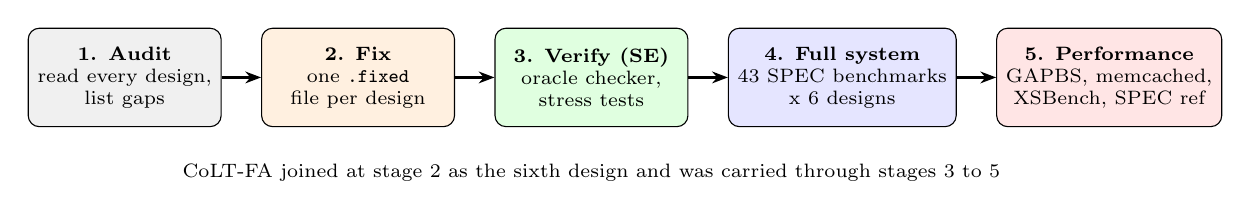
\begin{tikzpicture}[
  node distance=0.45cm and 0.5cm,
  box/.style={draw, rounded corners, fill=#1, minimum width=2.45cm, minimum height=1.25cm, align=center, font=\scriptsize},
  box/.default=blue!8,
  arr/.style={-{Stealth[length=2mm]}, thick}]
\node[box=gray!12] (a) {\textbf{1. Audit}\\read every design,\\list gaps};
\node[box=orange!12, right=of a] (b) {\textbf{2. Fix}\\one \texttt{.fixed}\\file per design};
\node[box=green!12, right=of b] (c) {\textbf{3. Verify (SE)}\\oracle checker,\\stress tests};
\node[box=blue!10, right=of c] (d) {\textbf{4. Full system}\\43 SPEC benchmarks\\x 6 designs};
\node[box=red!10, right=of d] (e) {\textbf{5. Performance}\\GAPBS, memcached,\\XSBench, SPEC ref};
\draw[arr] (a) -- (b); \draw[arr] (b) -- (c); \draw[arr] (c) -- (d); \draw[arr] (d) -- (e);
\node[below=0.35cm of c, font=\scriptsize, text width=11cm, align=center] {CoLT-FA joined at stage 2 as the sixth design and was carried through stages 3 to 5};
\end{tikzpicture}
\caption{Stages of the second phase.}
\label{fig:phase2_flow}
\end{figure}

Table~\ref{tab:designs} lists the six designs evaluated in this phase. All of them keep the 64-entry L1 TLB and the 128-set, 4-way L2 TLB with XOR-7 indexing from Part~\ref{part:mid}, unless a design changes the L2 itself.

\begin{table}[htbp]
\centering
\small
\caption{The six L2 TLB designs evaluated in the second phase.}
\label{tab:designs}
\begin{tabularx}{\textwidth}{l l X}
\toprule
\textbf{Design} & \textbf{Source files} & \textbf{What it does} \\
\midrule
Inclusive & \texttt{tlb.\{cc,hh\}.inc.fixed} & Every L1 entry also lives in the L2 (Section~3.2.1). \\
Exclusive & \texttt{tlb.\{cc,hh\}.excl.fixed} & A translation lives in only one level; L2 hits are promoted, L1 victims spill to L2. \\
NINE & \texttt{tlb.\{cc,hh\}.nine.fixed} & L1 and L2 are filled independently. \\
Agile / NaiveFP & \texttt{tlb.\{cc,hh\}.agile.fixed} & NINE plus a prefetcher that installs neighbouring translations, now with runtime parameters. \\
Perforated Pages & \texttt{tlb.\{cc,hh\}.perf.fixed} & L2 entries cover 2MB regions with a validity bitmap and a coarse filter (Section~6). \\
CoLT-FA & \texttt{tlb.\{cc,hh\}.colt.fixed} & NINE plus an 8-entry fully associative buffer of coalesced runs of up to 8 pages (Section~\ref{sec:colt_fs}). \\
\bottomrule
\end{tabularx}
\end{table}

% -----------------------------------------------------------------------------
\section{Implementation Audit}
\label{sec:audit}
% -----------------------------------------------------------------------------

The first task was a line-by-line audit of every TLB variant from Part~\ref{part:mid} (recorded in \texttt{TLB\_IMPLEMENTATION\_AUDIT.md}). The audit found problems in how the designs were built and tested, and also in what the code did when an operating system is present. Table~\ref{tab:audit} summarises the findings.

\begin{table}[htbp]
\centering
\small
\caption{Main findings of the implementation audit.}
\label{tab:audit}
\begin{tabularx}{\textwidth}{l X X}
\toprule
\textbf{\#} & \textbf{Finding} & \textbf{Why it matters} \\
\midrule
1 & The policy files were snapshots (for example \texttt{tlb.cc.inclusive.sa}). Only \texttt{tlb.cc} is compiled, so a design was only active if its snapshot was copied over \texttt{tlb.cc} before the build. & It was easy to measure a different design from the one intended. Each design now has its own build. \\
2 & The L2 was not invalidated when the kernel unmaps a page (\texttt{demapPage}) or switches address space (\texttt{flushNonGlobal} on a CR3 write) in several designs. & A stale L2 entry could hand out an old physical address after the page was freed or remapped. \\
3 & The L2 removal function matched entries by virtual address only and ignored the PCID stored in the low 12 bits of the key. & An unmap in one process could remove another process's entry, or miss its own. \\
4 & \texttt{serialize}/\texttt{unserialize} saved only the L1 array. & After a checkpoint restore the L2 state was silently lost. \\
5 & The Perforated Pages and Agile prefetch code were not integrated into a buildable, testable form, and the Agile prefetcher cited the wrong paper. & Results could not be reproduced. The citation was corrected to Vavouliotis et al.~\cite{vavouliotis2021agile}. \\
6 & No test compared the TLB's answer with the true page table. Results were raw miss counts. & A design that returns wrong translations can still show fewer misses. \\
\bottomrule
\end{tabularx}
\end{table}

An important point from the audit is that findings 2 and 3 cannot be triggered in SE mode. In SE mode \texttt{gem5} never calls \texttt{demapPage}, because it is only reached from full-system code paths (the page fault handler and the \texttt{INVLPG} instruction), and it always uses PCID 0. This is why the second phase had to move to full-system simulation (Section~\ref{sec:fs_method}).

% -----------------------------------------------------------------------------
\section{Correctness Fixes for Each Design}
\label{sec:fixes}
% -----------------------------------------------------------------------------

Each design was fixed in a new source file (\texttt{tlb.cc.<design>.fixed} and \texttt{tlb.hh.<design>.fixed}), so the original snapshots stay unchanged for comparison. The fixes common to all designs are listed first, followed by the design-specific ones.

\subsection{Fixes Common to All Designs}
\begin{itemize}
    \item \textbf{L2 invalidation on unmap}: \texttt{demapPage(va, asn)} now also removes the matching L2 entry.
    \item \textbf{L2 invalidation on address-space switch}: \texttt{flushNonGlobal()} now clears every non-global L2 entry, as it already did for the L1.
    \item \textbf{PCID-aware removal}: \texttt{l2\_remove} now builds the same \texttt{concAddrPcid(vpn, pcid)} key that \texttt{l2\_insert} uses, so only the translation of the right address space is removed.
    \item \textbf{Checkpointing}: the L2 contents are saved and restored together with the L1 (Perforated Pages clears the L2 on restore instead).
    \item \textbf{Statistics}: new counters for L2 hits, insertions and evictions (\texttt{l2Hits}, \texttt{l2Insertions}, \texttt{l2Evictions}).
    \item \textbf{Runtime parameters}: L2 geometry, hash function and replacement policy can be chosen with environment variables, so one binary can be used for a whole parameter sweep without rebuilding.
\end{itemize}

\subsection{Design-Specific Fixes}

\paragraph{Inclusive.} Four issues were fixed (Table~\ref{tab:inc_bugs}). While fixing the checkpoint code we also found that \texttt{gem5}'s checkpoint format is positional: a value written after a group of entries is read back as part of that group. The first two attempts at the fix failed on restore for this reason, and the third attempt placed all L2 values in their own section.

\begin{table}[htbp]
\centering
\small
\caption{Inclusive design: issues found and fixed.}
\label{tab:inc_bugs}
\begin{tabularx}{\textwidth}{l X X}
\toprule
\textbf{\#} & \textbf{Issue} & \textbf{Fix} \\
\midrule
1 & \texttt{l2\_remove(va)} ignored the PCID. & Removal uses the full \texttt{(va, pcid)} key. \\
2 & Checkpoints held only the L1 (a checkpoint taken after a 2,048-page run had 64 L1 entries and no L2 keys). & L2 sets and entries are serialized. \\
3 & Checkpoint values placed after the entry list were read back in the wrong section. & L2 state written in its own section. \\
4 & L2 geometry, hash and replacement were compile-time constants. & Selectable at runtime (\texttt{TLB\_L2\_GEOM}, \texttt{TLB\_L2\_HASH}, \texttt{TLB\_L2\_REPL}, \texttt{TLB\_L1\_SIZE}). \\
\bottomrule
\end{tabularx}
\end{table}

\paragraph{Exclusive.} The exclusive policy requires that a translation is never in both levels at once. We added a checker for this rule. With several hardware threads sharing the TLB (SMT), promotion and eviction could leave duplicate translations: the checker recorded \textbf{391,950 duplicate violations in 1,368,154 checks} on the original code. After the fix the same run reports \textbf{0} violations. The PCID-aware removal and the L2 checkpointing were fixed as for the other designs.

\paragraph{NINE.} The same PCID and checkpoint issues were fixed. Since NINE has no inclusion rule to check, a \emph{staleness scan} was added instead: after every flush, unmap and checkpoint restore, every valid L1 and L2 entry is checked again against the page table. On the \texttt{remap} stress test the scan ran 30 times and found no stale entry.

\paragraph{Agile / NaiveFP.} Seven issues were fixed in the prefetching design (Table~\ref{tab:agile_bugs}). The prefetcher was also turned into a runtime-parameterised design (degree, direction, adaptive degree, throttling and priority are selected with \texttt{AGILE\_PF\_*} variables) with counters for issued, useful and unused prefetches.

\begin{table}[htbp]
\centering
\small
\caption{Agile / NaiveFP design: issues found and fixed.}
\label{tab:agile_bugs}
\begin{tabularx}{\textwidth}{l X}
\toprule
\textbf{\#} & \textbf{Issue} \\
\midrule
1 & \texttt{l2\_remove()} was declared in the header but never defined. \\
2 & \texttt{demapPage()} never touched the L2. \\
3 & \texttt{demapPage()} looked up the L1 with the raw address instead of the PCID-tagged key. \\
4 & \texttt{flushNonGlobal()} never touched the L2. \\
5 & Checkpoints never saved or restored the L2. \\
6 & No prefetch counters, so useful prefetches could not be told apart from wasted ones. \\
7 & In our own adaptive-degree code, the degree was reset on every window boundary, even after a successful window (found and fixed during the campaign). \\
\bottomrule
\end{tabularx}
\end{table}

\paragraph{Perforated Pages.} Six issues were fixed (Table~\ref{tab:perf_bugs}). Issue 4 is the most serious: every L2 hit returned a translation with hard-coded permissions (user access allowed, execution allowed), so in full-system mode a user program could have been given access to a kernel page.

\begin{table}[htbp]
\centering
\small
\caption{Perforated Pages design: issues found and fixed.}
\label{tab:perf_bugs}
\begin{tabularx}{\textwidth}{l X X}
\toprule
\textbf{\#} & \textbf{Issue} & \textbf{Fix} \\
\midrule
1 & \texttt{demapPage()} cleared only the L1, so the L2 kept a stale sub-page. & Also clears the sub-page in the L2 and updates its coarse filter. \\
2 & \texttt{flushNonGlobal()} cleared only the L1. & Also clears non-global L2 regions. \\
3 & L2 regions had no address-space tag. & A \texttt{pcid} field is part of the match. \\
4 & L2 hits were rebuilt with hard-coded \texttt{user=true}, \texttt{noExec=false}, \texttt{global=false}. & The real per-page permissions are stored and returned. \\
5 & On every SE miss, \texttt{l2\_insert()} was called twice for the same page. & The extra call was removed. \\
6 & Checkpoints never touched the L2. & The L2 is cleared on restore. \\
\bottomrule
\end{tabularx}
\end{table}

\paragraph{CoLT-FA.} CoLT-FA needed the most work and is described in its own section (Section~\ref{sec:colt_fs}).

% -----------------------------------------------------------------------------
\section{Verification Framework}
\label{sec:verif}
% -----------------------------------------------------------------------------

\subsection{Translation Oracle and Invariant Checkers}
To check correctness instead of only counting misses, we added an instrumentation layer to \texttt{tlb.cc}. It is applied by a script (\texttt{robustness/patches/apply\_checker*.py}) so that the same checker is used for every design:
\begin{itemize}
    \item \textbf{Translation oracle}: every time a translation finishes, the physical address given by the TLB is compared with the true one. In SE mode the true answer comes from the process page table. In full-system mode the checker does its own functional page walk of the guest page table every $N$-th translation ($N = 64$ by default, set with \texttt{TLBCHK\_FS\_PERIOD}).
    \item \textbf{Inclusion invariant} (Inclusive): every valid L1 entry must have a matching L2 entry.
    \item \textbf{Exclusivity invariant} (Exclusive): no translation may be valid in both levels.
    \item \textbf{Staleness scan} (NINE, CoLT-FA): after every flush, unmap and restore, every valid entry is re-checked against the page table.
\end{itemize}
Mismatches are counted in \texttt{stats.txt} (\texttt{chkOracleMismatch}, \texttt{chkOracleWalkFault}, \texttt{chkStaleL1}, \texttt{chkStaleL2}) and the first few are printed with details.

\subsection{Stress Tests}
Three test programs were written for the SE-mode matrix (\texttt{robustness/tests/}):
\begin{itemize}
    \item \texttt{tlbstress}: capacity, set-conflict, remap, protection change, huge page, TLB shootdown, multi-thread, multi-process, interrupt and shared-memory tests.
    \item \texttt{pf\_patterns}: nine access patterns (ascending, descending, strides 2/4/8/16, random, pointer chasing, hot/cold) over a chosen number of pages.
    \item \texttt{perf\_holes}: 2MB regions with different hole patterns (dense, edge, clustered, dispersed, one hole per 64 pages, sparse, churn) for Perforated Pages.
\end{itemize}
These were combined into a job matrix covering Atomic, Timing and O3 CPUs, single and multiple cores, multi-threaded and multi-programmed runs, SMT with 2 and 4 threads, and fork with shared memory. Every job was run on the design under test \emph{and} on stock \texttt{gem5}, so a failure that also happens on stock \texttt{gem5} can be separated from a failure of the design.

\subsection{Problems in the Test Harness}
Two harness problems were found and fixed while setting up SPEC CPU2017 in SE mode:
\begin{itemize}
    \item \texttt{gem5}'s SE configuration redirects any guest path under \texttt{/tmp} into its own output directory. Since the SPEC installation was under \texttt{/tmp}, SPEC could not find its own files. The installation was moved to \texttt{/var/tmp}.
    \item Some SPEC benchmarks take options that start with a dash (for example \texttt{-I./lib} for perlbench), which \texttt{se.py} tried to read as its own options. The job generator was changed to pass the options as a single argument.
\end{itemize}

% -----------------------------------------------------------------------------
\section{SE-Mode Verification Results}
\label{sec:se_results}
% -----------------------------------------------------------------------------

\subsection{Correctness Matrix}
Table~\ref{tab:se_matrix} gives the SE-mode results. \textbf{No design produced a single oracle mismatch.} Every failure in the matrix also fails, in the same way, on stock \texttt{gem5}: these are known limits of SE mode (\texttt{setitimer} not implemented, fork with \texttt{MAP\_SHARED} hanging past the timeout, and multi-process remap tests that see stale data on stock \texttt{gem5} too).

\begin{table}[htbp]
\centering
\small
\caption{SE-mode correctness results. "Same on stock" means every failing job also fails identically on unmodified \texttt{gem5}.}
\label{tab:se_matrix}
\begin{tabularx}{\textwidth}{l l l X}
\toprule
\textbf{Design} & \textbf{Matrix} & \textbf{Oracle mismatches} & \textbf{Notes} \\
\midrule
Inclusive & 94/120 (original), 47/54 (fixed) & 0 & 26 failures, all same on stock; 0 inclusion violations \\
Exclusive & 94/120 & 0 & all 26 failures same on stock; duplicate violations 391,950 $\rightarrow$ 0 \\
NINE & 94/120 (original), 47/57 (fixed) & 0 & 0 design-specific failures; staleness scan found 0 stale entries \\
Agile / NaiveFP & 20/24 tlbstress, 108/108 \texttt{pf\_patterns} & 0 & the 4 failures (shared memory) hang on stock too \\
Perforated Pages & 36/44 & 0 & the 8 non-passes identical on stock; 31 configurations swept \\
CoLT-FA & 36/36 & 0 & see Section~\ref{sec:colt_se} \\
\bottomrule
\end{tabularx}
\end{table}

\subsection{SPEC CPU2017 in SE Mode}
For the Inclusive design, all SPEC CPU2017 rate benchmarks that could be built were run with test inputs on the Atomic CPU, on both the fixed design and stock \texttt{gem5}, with the oracle and inclusion checker turned on. \textbf{All 31 SPEC invocations that could run passed, with 0 inclusion violations, 0 oracle mismatches and output identical to stock \texttt{gem5}.} The two that could not run (perlbench and omnetpp) failed on both builds because of the option problem described above.

\subsection{Design Parameter Sweeps}
Because the fixed designs take their parameters at runtime, each design was swept with a single binary. All variants kept 0 correctness errors. Tables~\ref{tab:sweep_inc} to~\ref{tab:sweep_perf} show selected rows.

\begin{table}[htbp]
\centering
\small
\caption{Inclusive design: selected variants (adversarial set-conflict benchmark, Atomic CPU). L2 hits and back-invalidations of the L1 caused by L2 evictions.}
\label{tab:sweep_inc}
\begin{tabular}{l c c c r r}
\toprule
\textbf{Variant} & \textbf{Geometry} & \textbf{Hash} & \textbf{Repl.} & \textbf{L2 hits} & \textbf{Back-inval.} \\
\midrule
Default & 128$\times$4 & XOR-7 & LRU & 0 & 3,130 \\
Geometry 64$\times$8 & 64$\times$8 & XOR-7 & LRU & 1,973 & 0 \\
Geometry 256$\times$2 & 256$\times$2 & XOR-7 & LRU & 1,925 & 20 \\
Fully associative & 1$\times$512 & XOR-7 & LRU & 1,973 & 0 \\
Modulo hash & 128$\times$4 & modulo & LRU & 1,973 & 0 \\
XOR-fold hash & 128$\times$4 & XOR-fold & LRU & 0 & 3,030 \\
Random replacement & 128$\times$4 & XOR-7 & random & 0 & 3,151 \\
\bottomrule
\end{tabular}
\end{table}

\begin{table}[htbp]
\centering
\small
\caption{Exclusive design: selected variants. TLB misses of the design against stock \texttt{gem5} (36,348 misses).}
\label{tab:sweep_excl}
\begin{tabular}{l l r r}
\toprule
\textbf{Variant} & \textbf{Setting} & \textbf{Misses} & \textbf{Change vs stock} \\
\midrule
Default & 128 sets, 4 ways, XOR-7, LRU, always spill & 9,063 & $-75.1\%$ \\
Sets 64 & \texttt{EXCL\_L2\_SETS=64} & 23,491 & $-35.4\%$ \\
Sets 256 & \texttt{EXCL\_L2\_SETS=256} & 5,891 & $-83.8\%$ \\
Ways 2 & \texttt{EXCL\_L2\_WAYS=2} & 26,658 & $-26.7\%$ \\
Modulo hash & \texttt{EXCL\_L2\_HASH=1} & 6,114 & $-83.2\%$ \\
Dirty-hot spill & \texttt{EXCL\_SPILL=dirty-hot} & 36,244 & $-0.3\%$ \\
No spill & \texttt{EXCL\_SPILL=never} & 36,348 & $0.0\%$ \\
Smaller L1 & \texttt{EXCL\_L1\_SIZE=32} & 9,260 & $-74.5\%$ \\
\bottomrule
\end{tabular}
\end{table}

\begin{table}[htbp]
\centering
\small
\caption{NINE design: selected variants (L1 misses and L2 hits on the same workload).}
\label{tab:sweep_nine}
\begin{tabular}{l l r r r}
\toprule
\textbf{Variant} & \textbf{Setting} & \textbf{L2 entries} & \textbf{L1 misses} & \textbf{L2 hits} \\
\midrule
Default & none & 512 & 48,727 & 2,624 \\
Sets 64 & \texttt{NINE\_L2\_SETS=64} & 256 & 50,587 & 764 \\
Sets 256 & \texttt{NINE\_L2\_SETS=256} & 1,024 & 41,763 & 9,588 \\
Ways 2 & \texttt{NINE\_L2\_WAYS=2} & 256 & 50,576 & 775 \\
Ways 8 & \texttt{NINE\_L2\_WAYS=8} & 1,024 & 42,395 & 8,956 \\
Low-bits hash & \texttt{NINE\_L2\_HASH=1} & 512 & 48,003 & 3,348 \\
Random replacement & \texttt{NINE\_L2\_REPL=2} & 512 & 47,832 & 3,519 \\
\bottomrule
\end{tabular}
\end{table}

\noindent For NINE, doubling the total L2 capacity (more sets or more ways) roughly doubled the L2 hit rate, while the hash and replacement choice made a smaller difference at a fixed capacity.

\begin{table}[htbp]
\centering
\small
\caption{Agile prefetcher: selected variants (2,048 pages, 3 passes). Walks, issued prefetches, useful prefetches, and prefetches evicted unused (pollution).}
\label{tab:sweep_agile}
\begin{tabular}{l l r r r r}
\toprule
\textbf{Pattern} & \textbf{Variant} & \textbf{Walks} & \textbf{Issued} & \textbf{Useful} & \textbf{Unused} \\
\midrule
ascending & degree 1 & 4,919 & 20,041 & 5,436 & 52 \\
ascending & degree 4 & 4,324 & 70,308 & 6,031 & 172 \\
ascending & degree 8 & 4,224 & 136,584 & 6,131 & 236 \\
ascending & adaptive (exp) & 4,238 & 21,490 & 6,117 & 164 \\
ascending & degree 4, wrong direction & 10,287 & 263,392 & 68 & 177 \\
random & degree 1 & 9,054 & 48,986 & 1,305 & 32,430 \\
random & degree 8 & 8,767 & 422,793 & 1,601 & 289,525 \\
\bottomrule
\end{tabular}
\end{table}

\noindent For the Agile prefetcher, the adaptive degree reached almost the same number of walks as a fixed degree of 8 on the ascending pattern (4,238 against 4,224) while issuing about one sixth of the prefetches (21,490 against 136,584). On the random pattern most prefetches were never used.

\begin{table}[htbp]
\centering
\small
\caption{Perforated Pages: selected variants out of 31 (total L1 misses, one knob changed at a time).}
\label{tab:sweep_perf}
\begin{tabular}{l l r r}
\toprule
\textbf{Variant} & \textbf{Setting} & \textbf{L1 misses} & \textbf{vs baseline} \\
\midrule
Baseline & 128 sets, 4 ways, 8 chunks, prefetch 8, LRU & 149,703 & -- \\
All four fixes reverted & \texttt{PERF\_FIX\_*=0} & 149,703 & $+0.0\%$ \\
16 sets, 1 way & \texttt{PERF\_L2\_SETS=16 PERF\_L2\_WAYS=1} & 159,810 & $+6.8\%$ \\
1 set, 1 way & \texttt{PERF\_L2\_SETS=1 PERF\_L2\_WAYS=1} & 189,673 & $+26.7\%$ \\
No prefetch & \texttt{PERF\_PREFETCH\_DEGREE=1} & 242,905 & $+62.3\%$ \\
Prefetch 64 (best) & \texttt{PERF\_PREFETCH\_DEGREE=64} & 136,601 & $-8.8\%$ \\
\bottomrule
\end{tabular}
\end{table}

\noindent For Perforated Pages, reverting the four correctness fixes did not change the SE-mode miss count, which is expected: the paths they fix are not reached in SE mode.

% -----------------------------------------------------------------------------
\section{CoLT-FA Rebuilt for Full-System Simulation}
\label{sec:colt_fs}
% -----------------------------------------------------------------------------

\subsection{Why the Mid-Review CoLT-FA Did Not Work Under an Operating System}
The CoLT-FA buffer from Section~5 found contiguous pages by reading \texttt{gem5}'s \emph{emulated} page table (\texttt{p->pTable->lookup}). This table only exists in SE mode. In full-system mode the operating system owns the page tables and \texttt{gem5}'s hardware page walker reads them from simulated memory, so the mid-review CoLT-FA never formed a single coalesced entry. It also had the same problems as the other designs: entries had no PCID, the permissions of every hit were fixed in the code (\texttt{user=true}, \texttt{noExec=false}), and nothing cleared the buffer on an unmap or an address-space switch.

\subsection{New Design}
We rebuilt CoLT-FA on top of the fixed NINE L2 (\texttt{tlb.cc.nine.fixed}), which was the baseline used for CoLT in Part~\ref{part:mid}. The changes are generated by one script (\texttt{robustness/patches/make\_colt\_fixed.py}) that writes \texttt{tlb.cc.colt.fixed}, \texttt{tlb.hh.colt.fixed} and \texttt{pagetable\_walker.cc.colt}.

\begin{itemize}
    \item \textbf{Coalescing in the page walker.} As in the CoLT paper, coalescing now happens when a walk reads the final 4KB page table entry. That entry sits in a 64-byte cache line together with seven neighbouring entries. The walker reads this line and passes the eight entries to the TLB (\texttt{coltObserveLeaf}).
    \item \textbf{Forming a run.} Starting from the requested page, the TLB extends the run backwards and forwards as long as the next entry is present, has the same permission and caching bits (present, writable, user, PWT, PCD, PAT, global, no-execute), and points to the next physical page. A run of 2 to 8 pages is inserted into the buffer.
    \item \textbf{Buffer.} 8 fully associative entries by default (\texttt{COLT\_FA\_ENTRIES}), LRU replacement, each entry tagged with its PCID and holding the real permissions from the walk.
    \item \textbf{Lookup order.} L1, then the CoLT-FA buffer, then the L2, then a page walk.
    \item \textbf{Invalidation.} The buffer is cleared on \texttt{flushAll}, non-global entries are cleared on \texttt{flushNonGlobal}, any run covering the address is removed on \texttt{demapPage}, and the buffer starts empty after a checkpoint restore.
    \item \textbf{Same binary as the baseline.} \texttt{COLT\_ENABLE=0} turns the buffer off, so the same \texttt{gem5} binary also runs plain NINE. This makes it possible to compare CoLT-FA and NINE with everything else held equal.
\end{itemize}

Figure~\ref{fig:colt_flow} shows the new flow.

\begin{figure}[htbp]
\centering
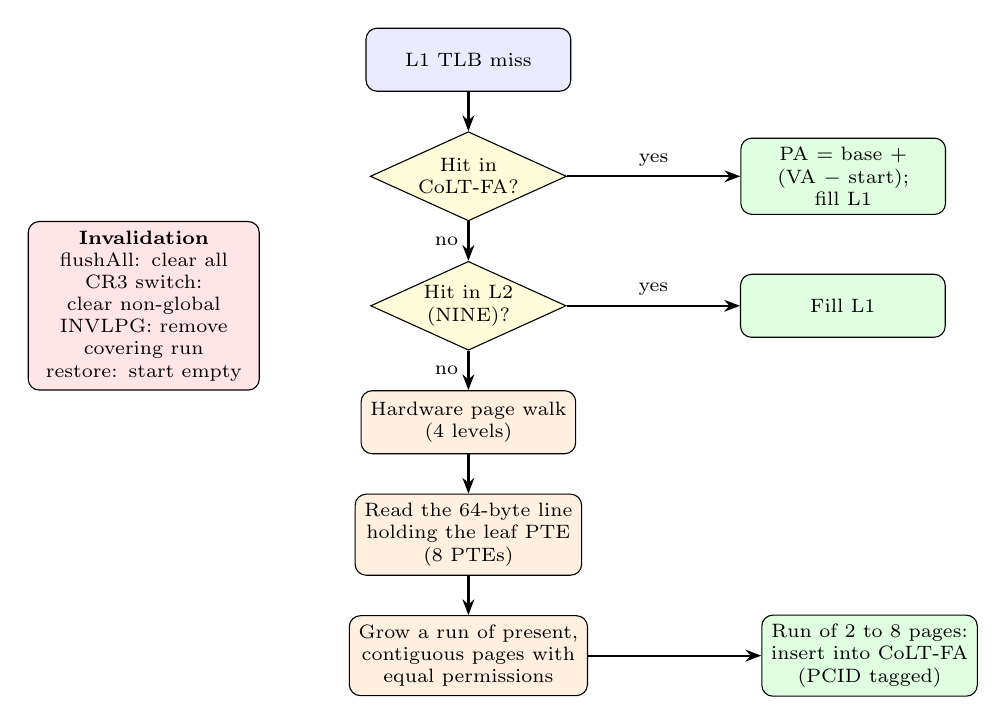
\begin{tikzpicture}[
  node distance=0.5cm and 0.6cm,
  st/.style={draw, rounded corners, fill=#1, align=center, font=\scriptsize, minimum width=2.6cm, minimum height=0.8cm},
  st/.default=blue!8,
  dec/.style={draw, diamond, aspect=2.2, fill=yellow!15, align=center, font=\scriptsize, inner sep=1pt},
  arr/.style={-{Stealth[length=2mm]}, thick}]
\node[st] (miss) {L1 TLB miss};
\node[dec, below=of miss] (colt) {Hit in\\CoLT-FA?};
\node[dec, below=of colt] (l2) {Hit in L2\\(NINE)?};
\node[st=orange!12, below=of l2] (walk) {Hardware page walk\\(4 levels)};
\node[st=orange!12, below=of walk] (line) {Read the 64-byte line\\holding the leaf PTE\\(8 PTEs)};
\node[st=orange!12, below=of line] (run) {Grow a run of present,\\contiguous pages with\\equal permissions};
\node[st=green!12, right=2.2cm of colt] (fill1) {PA = base +\\(VA $-$ start);\\fill L1};
\node[st=green!12, right=2.2cm of l2] (fill2) {Fill L1};
\node[st=green!12, right=2.2cm of run] (ins) {Run of 2 to 8 pages:\\insert into CoLT-FA\\(PCID tagged)};
\draw[arr] (miss) -- (colt);
\draw[arr] (colt) -- node[left, font=\scriptsize]{no} (l2);
\draw[arr] (l2) -- node[left, font=\scriptsize]{no} (walk);
\draw[arr] (walk) -- (line);
\draw[arr] (line) -- (run);
\draw[arr] (colt) -- node[above, font=\scriptsize]{yes} (fill1);
\draw[arr] (l2) -- node[above, font=\scriptsize]{yes} (fill2);
\draw[arr] (run) -- (ins);
\node[st=red!10, left=1.4cm of l2, text width=2.7cm] (inv) {\textbf{Invalidation}\\flushAll: clear all\\CR3 switch: clear non-global\\INVLPG: remove covering run\\restore: start empty};
\end{tikzpicture}
\caption{Lookup and coalescing flow of the rebuilt CoLT-FA design in full-system mode.}
\label{fig:colt_flow}
\end{figure}

Two details were decided on purpose. First, the accessed and dirty bits are not compared when forming a run: the accessed bit of the requested entry is only written back after this step, and \texttt{gem5}'s walker does not set the dirty bit at all, so comparing them would stop almost every run. Second, the checker described in Section~\ref{sec:verif} was applied to the CoLT-FA tree as well, so every CoLT-FA full-system run also checks one in every 64 translations against a functional page walk.

\subsection{SE-Mode Verification of CoLT-FA}
\label{sec:colt_se}
CoLT-FA was first checked in SE mode with 9 programs, on the Atomic and Timing CPUs, with CoLT turned on and off: 36 runs in total. \textbf{All 36 runs passed with 0 oracle mismatches and 0 stale entries.} Table~\ref{tab:colt_se} shows how active the buffer was on the Atomic CPU.

\begin{table}[htbp]
\centering
\small
\caption{CoLT-FA SE-mode verification (Atomic CPU). CoLT hits are L1 misses answered by the buffer; runs inserted are coalesced entries created.}
\label{tab:colt_se}
\begin{tabular}{l c r r r r}
\toprule
\textbf{Program} & \textbf{Result} & \textbf{CoLT hits} & \textbf{Runs inserted} & \textbf{L2 hits (off)} & \textbf{L2 hits (on)} \\
\midrule
\texttt{pf\_patterns} ascending, 16MB & PASS & 14,322 & 5,664 & 0 & 0 \\
\texttt{tlb\_colt\_bench} (8MB) & completed & 7,670 & 4,354 & 71 & 39 \\
\texttt{tlbstress} capacity 513 & PASS & 2,665 & 572 & 23,410 & 21,002 \\
\texttt{tlbstress} remap & PASS & 2,475 & 1,755 & 3,764 & 1,307 \\
\texttt{pf\_patterns} random, 16MB & PASS & 295 & 19,649 & 43 & 43 \\
\texttt{pf\_patterns} stride 8, 16MB & PASS & 263 & 4,089 & 15,730 & 15,606 \\
\texttt{tlbstress} conflict & PASS & 23 & 7 & 32 & 21 \\
\bottomrule
\end{tabular}
\end{table}

\noindent The buffer is most useful when pages are touched in address order (14,322 hits on the ascending pattern) and least useful on random access. The Timing CPU runs gave the same counts.

% -----------------------------------------------------------------------------
\section{Full-System Evaluation Methodology}
\label{sec:fs_method}
% -----------------------------------------------------------------------------

\subsection{Simulated System}
Table~\ref{tab:fs_setup} lists the simulated system. The configuration script \texttt{robustness/scripts/fs\_run.py} uses the \texttt{gem5} standard library \texttt{X86Board}.

\begin{table}[htbp]
\centering
\small
\caption{Full-system configuration.}
\label{tab:fs_setup}
\begin{tabularx}{\textwidth}{l X}
\toprule
\textbf{Item} & \textbf{Value} \\
\midrule
Simulator & \texttt{gem5} 25.1.0.1, x86, built with gcc-11 \\
Board & \texttt{X86Board}, 3 GiB guest memory (the largest this board supports), 1 core \\
Guest & Ubuntu 24.04, Linux kernel 6.8.0-52 \\
Caches & private L1 instruction and data caches and a private L2 cache \\
CPUs & atomic CPU for boot and most execution; timing CPU for measurement windows \\
TLB & 64-entry L1 plus the design under test \\
Benchmarks & on a second disk image built from the SPEC CPU2017 installation, mounted by the guest \\
Control & \texttt{gem5-bridge} hypercalls from the guest to the simulator \\
\bottomrule
\end{tabularx}
\end{table}

\subsection{Measurement Windows}
Running whole benchmarks on the detailed timing CPU was far too slow for the time available. Each benchmark therefore runs on the atomic CPU, which still uses the TLB under test for every access and so still tests correctness, and only a fixed \emph{window} of instructions is measured on the timing CPU. SPEC's own \texttt{submit} setting wraps every benchmark command with two hypercalls, so \texttt{gem5} knows when the benchmark program itself starts and ends (and not SPEC's setup scripts). Figure~\ref{fig:window} shows the sequence.

\begin{figure}[htbp]
\centering
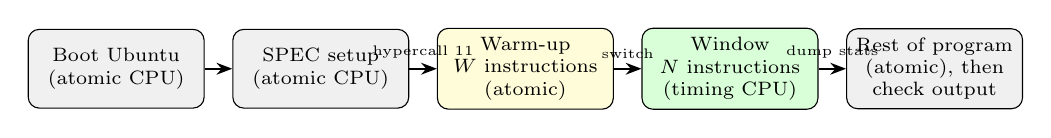
\begin{tikzpicture}[
  node distance=0.35cm and 0.35cm,
  ph/.style={draw, rounded corners, fill=#1, align=center, font=\scriptsize, minimum height=1.0cm, text width=2.0cm},
  arr/.style={-{Stealth[length=2mm]}, thick}]
\node[ph=gray!12] (boot) {Boot Ubuntu\\(atomic CPU)};
\node[ph=gray!12, right=of boot] (setup) {SPEC setup\\(atomic CPU)};
\node[ph=yellow!15, right=of setup] (warm) {Warm-up\\$W$ instructions\\(atomic)};
\node[ph=green!15, right=of warm] (meas) {Window\\$N$ instructions\\(timing CPU)};
\node[ph=gray!12, right=of meas] (rest) {Rest of program\\(atomic), then\\check output};
\draw[arr] (boot) -- (setup); \draw[arr] (setup) -- node[above, font=\tiny]{hypercall 11} (warm);
\draw[arr] (warm) -- node[above, font=\tiny]{switch} (meas); \draw[arr] (meas) -- node[above, font=\tiny]{dump stats} (rest);
\end{tikzpicture}
\caption{Measurement window for one benchmark. Hypercall 11 marks the start of the benchmark program and hypercall 12 its end.}
\label{fig:window}
\end{figure}

\begin{table}[htbp]
\centering
\small
\caption{Window settings used for each experiment.}
\label{tab:windows}
\begin{tabular}{l r r l}
\toprule
\textbf{Experiment} & \textbf{Warm-up $W$} & \textbf{Window $N$} & \textbf{After the window} \\
\midrule
SPEC CPU2017, test inputs & 50M & 200M & continue to the end, then SPEC checks the output \\
SPEC CPU2017, reference inputs & 3G & 200M & stop the simulation \\
GAPBS bfs, pr, cc, bc, tc & 250M & 1G & stop the simulation \\
GAPBS sssp & 300M & 800M & stop the simulation \\
XSBench & 2.6G & 500M & stop the simulation \\
STREAM & 100M & 500M & stop the simulation \\
memcached & GET phase only & 1.5G & stop the simulation \\
\bottomrule
\end{tabular}
\end{table}

If a program finishes before the window ends, the statistics up to that point are kept and marked as \emph{partial}. Short GAPBS kernels such as bfs and cc are measured this way in full.

\subsection{Running Several Hundred Simulations}
Each benchmark ran in its own \texttt{gem5} process. This made the runs independent, so a benchmark that crashes or fails does not affect any other. Over the campaign we used about 40 machines of the department lab. The flow is shown in Figure~\ref{fig:infra}. Since the lab machines could not reach GitHub, all code and tools were copied from a laptop, and the inputs (built \texttt{gem5}, kernel, Ubuntu image and SPEC tree, about 20GB per design) were copied from machine to machine. Each machine then built its own SPEC disk image with \texttt{mkfs.ext4 -d}. Results were copied back to the laptop every 30 minutes by \texttt{sync\_fs\_results.sh}.

\begin{figure}[htbp]
\centering
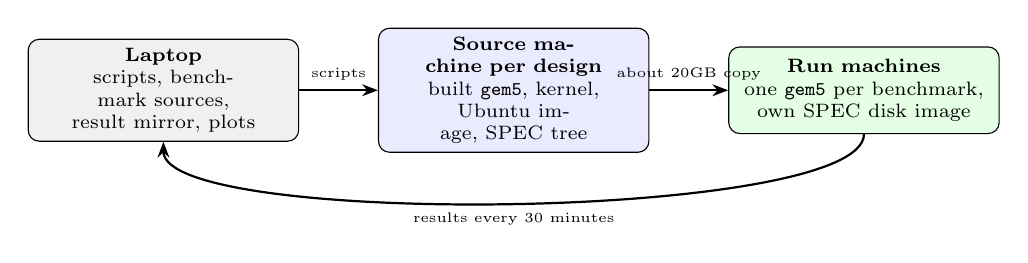
\begin{tikzpicture}[
  node distance=0.6cm and 1.0cm,
  bx/.style={draw, rounded corners, fill=#1, align=center, font=\scriptsize, text width=3.2cm, minimum height=1.1cm},
  arr/.style={-{Stealth[length=2mm]}, thick}]
\node[bx=gray!12] (lap) {\textbf{Laptop}\\scripts, benchmark sources,\\result mirror, plots};
\node[bx=blue!8, right=of lap] (src) {\textbf{Source machine per design}\\built \texttt{gem5}, kernel,\\Ubuntu image, SPEC tree};
\node[bx=green!10, right=of src] (run) {\textbf{Run machines}\\one \texttt{gem5} per benchmark,\\own SPEC disk image};
\draw[arr] (lap) -- node[above, font=\tiny]{scripts} (src);
\draw[arr] (src) -- node[above, font=\tiny]{about 20GB copy} (run);
\draw[arr] (run.south) .. controls +(0,-1.1) and +(0,-1.1) .. node[below, font=\tiny]{results every 30 minutes} (lap.south);
\end{tikzpicture}
\caption{How the simulations were spread over the lab machines.}
\label{fig:infra}
\end{figure}

\subsection{Problems Met During the Campaign}
Table~\ref{tab:campaign_issues} records the problems that affected the runs and what was done about them. We report them because some of them changed how the results must be read.

\begin{table}[htbp]
\centering
\small
\caption{Problems met during the full-system campaign.}
\label{tab:campaign_issues}
\begin{tabularx}{\textwidth}{X X}
\toprule
\textbf{Problem} & \textbf{What was done} \\
\midrule
The window handler was registered as a list, which \texttt{gem5} uses only once. The second instruction-count event (end of the window) fell to the default handler and ended the simulation. & Registered as a single function, which runs on every event. All runs were restarted with the fix. \\
A warm-up of 500M instructions was longer than some SPEC test inputs. & Warm-up lowered to 50M for the test inputs. \\
The home directory has a quota of about 10GB, too small to stage the inputs. & Inputs copied directly between lab machines. \\
Several lab machines were rebooted or became unreachable during the runs. & Runs moved to other machines; finished results had already been copied back. \\
KVM is only available to the user logged in at a machine's own screen, not over SSH. & Every boot used the atomic CPU (about 2 hours per boot under load). \\
Many \texttt{gem5} processes on one machine slow each other down. & Measured (below); long benchmarks rerun on lightly loaded machines. \\
\bottomrule
\end{tabularx}
\end{table}

On an idle machine one \texttt{gem5} process ran a test program at 2.23 million instructions per second. The same program on a machine running about 30 \texttt{gem5} processes ran at 0.58 million instructions per second, 3.8 times slower. A loaded machine still completed about 7 times more work in total, so most benchmarks were packed onto shared machines. The 9 longest benchmarks were also rerun with only 4 or 5 processes per machine so they could finish in time.

% -----------------------------------------------------------------------------
\section{Full-System SPEC CPU2017 Results}
\label{sec:fs_spec}
% -----------------------------------------------------------------------------

All 43 SPEC CPU2017 benchmarks were run with test inputs on all six designs. A benchmark counts as PASS only if SPEC's own output check passes. Figure~\ref{fig:spec_outcome} and Table~\ref{tab:spec_outcome} give the results.

\begin{figure}[htbp]
\centering
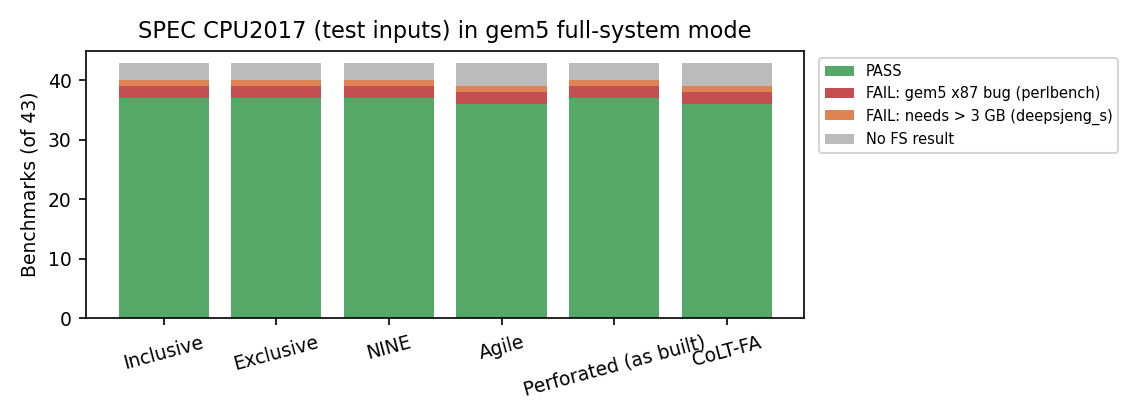
\includegraphics[width=\textwidth]{figures/spec_fs_outcome.png}
\caption{Outcome of the 43 SPEC CPU2017 benchmarks (test inputs) on each design in full-system mode.}
\label{fig:spec_outcome}
\end{figure}

\begin{table}[htbp]
\centering
\small
\caption{Full-system SPEC CPU2017 results (test inputs, out of 43).}
\label{tab:spec_outcome}
\begin{tabular}{l c c c c}
\toprule
\textbf{Design} & \textbf{PASS} & \textbf{FAIL: x87 bug} & \textbf{FAIL: memory} & \textbf{No full-system result} \\
\midrule
Inclusive & 37 & 2 & 1 & 3 \\
Exclusive & 37 & 2 & 1 & 3 \\
NINE & 37 & 2 & 1 & 3 \\
Agile / NaiveFP & 36 & 2 & 1 & 4 \\
Perforated Pages & 37 & 2 & 1 & 3 \\
CoLT-FA & 36 & 2 & 1 & 4 \\
\bottomrule
\end{tabular}
\end{table}

\begin{figure}[htbp]
\centering
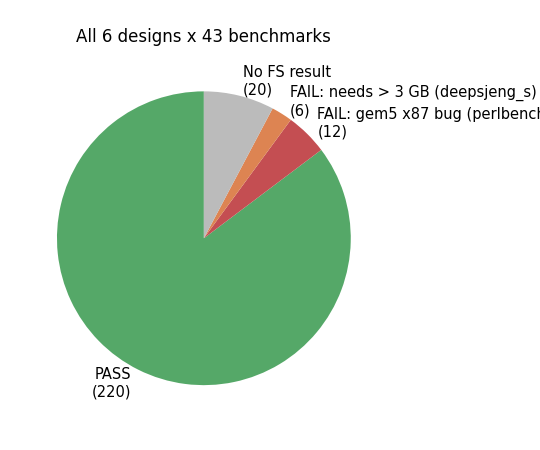
\includegraphics[width=0.45\textwidth]{figures/spec_fs_pie.png}
\caption{Outcome of all 258 benchmark runs (6 designs $\times$ 43).}
\label{fig:spec_pie}
\end{figure}

\noindent \textbf{Every benchmark that can run in this setup passes on every design.} The same three benchmarks fail on every design, and none of the failures depends on the TLB:
\begin{itemize}
    \item \textbf{500.perlbench\_r and 600.perlbench\_s} fail because of a bug in \texttt{gem5}'s emulation of x87 floating-point instructions. Perl prints long double values (\texttt{printf "\%a"}) through these instructions and the result is wrong under \texttt{gem5}. We checked that both benchmarks pass natively with the exact same SPEC setup and wrapper, and that they still fail in \texttt{gem5} with the wrapper removed. A patch to the x87 microcode was in progress at the time of writing.
    \item \textbf{631.deepsjeng\_s} needs 6.9GB of memory, more than the 3 GiB the board allows, so the program cannot start.
\end{itemize}

\noindent Four more benchmarks have no full-system pass/fail result:
\begin{itemize}
    \item \textbf{619.lbm\_s} needs 3.2GB, just above the memory limit, and \texttt{gem5} stops with an internal cache assertion when it switches back from the timing to the atomic CPU after its window. Its window statistics were saved.
    \item \textbf{525.x264\_r and 625.x264\_s} run about 1 trillion instructions each on the test input, which would take around 13 days to simulate. Their window statistics were saved.
    \item \textbf{627.cam4\_s} passes on four designs and was still running on Agile and CoLT-FA at the time of writing. It fails natively on our SPEC build but passes in \texttt{gem5}.
\end{itemize}

\subsection{The Two Large Benchmarks in SE Mode}
Since 631.deepsjeng\_s and 619.lbm\_s do not fit in the full-system guest, both were run in SE mode with 8 GiB of memory on all six designs. Each output was compared byte by byte with the native output, which had passed SPEC's check. 619.lbm\_s is an OpenMP program, so it was run with one OpenMP thread (\texttt{OMP\_NUM\_THREADS=1}).

\begin{table}[htbp]
\centering
\small
\caption{SE-mode results with 8 GiB of memory.}
\label{tab:se_bigmem}
\begin{tabular}{l c c c c c c}
\toprule
\textbf{Benchmark} & \textbf{Inclusive} & \textbf{Exclusive} & \textbf{NINE} & \textbf{Agile} & \textbf{Perforated} & \textbf{CoLT-FA} \\
\midrule
631.deepsjeng\_s & PASS & PASS & PASS & PASS & PASS & PASS \\
619.lbm\_s & PASS & PASS & PASS & PASS & PASS & PASS \\
\bottomrule
\end{tabular}
\end{table}

\noindent The CoLT-FA runs had the oracle turned on and reported 0 mismatches, with 1,600,771 buffer hits on 631.deepsjeng\_s and 62,071,327 on 619.lbm\_s.

\subsection{How Much the SPEC Test Inputs Use the TLB}
The windows also show how hard each benchmark pushes the TLB. Figure~\ref{fig:spec_pressure} plots the page walks per 1000 instructions on the Inclusive design. The highest value is 1.145 (638.imagick\_s), and benchmarks usually called memory-intensive stay low: 605.mcf\_s is 0.242, and lbm, roms and xz stay at or below about 0.5. The test inputs are small, so their working sets mostly fit in the TLB's reach. \textbf{The SPEC test-input runs are therefore mainly a correctness result}, and the performance comparison in Section~\ref{sec:perf} uses workloads that stress the TLB much more.

\begin{figure}[htbp]
\centering
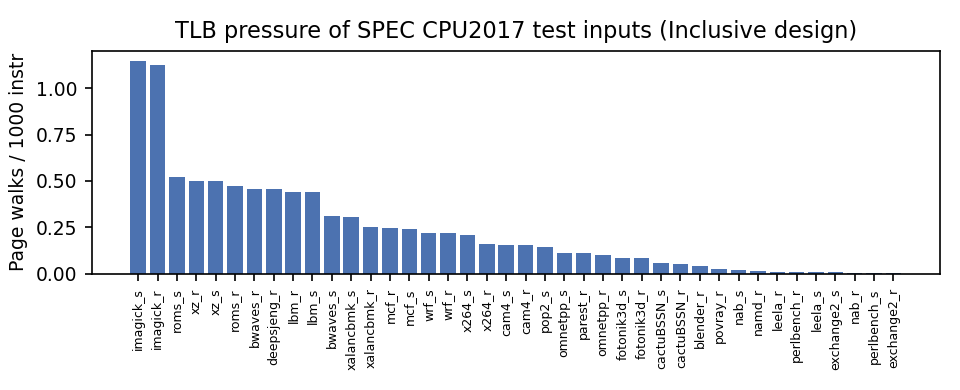
\includegraphics[width=\textwidth]{figures/spec_test_pressure.png}
\caption{Page walks per 1000 instructions for the SPEC CPU2017 test inputs (Inclusive design, 200M-instruction window).}
\label{fig:spec_pressure}
\end{figure}

% -----------------------------------------------------------------------------
\section{Performance on TLB-Intensive Workloads}
\label{sec:perf}
% -----------------------------------------------------------------------------

\subsection{Workloads}
Following the instructor's suggestion, we used the GAPBS graph benchmark suite and a key-value store, together with other standard memory-intensive programs (Table~\ref{tab:workloads}). All programs were built as static binaries and placed on a separate disk image. The GAPBS graphs were generated once in advance with GAPBS's own converter, because generating the graph took about 95\% of the instructions of a bfs run. The memcached load generator (\texttt{mc-crusher}) does not stop by itself after a fixed number of requests, so a small driver script (\texttt{run\_memcached.sh}) watches memcached's own counters and stops each phase.

\begin{table}[htbp]
\centering
\small
\caption{TLB-intensive workloads. Native data-TLB misses per 1000 instructions were measured with \texttt{perf} on a lab machine (Intel, transparent huge pages in \texttt{madvise} mode).}
\label{tab:workloads}
\begin{tabularx}{\textwidth}{l X r r}
\toprule
\textbf{Workload} & \textbf{Configuration} & \textbf{Memory} & \textbf{Native misses / 1k instr} \\
\midrule
GAPBS bfs~\cite{beamer2015gap} & Kronecker graph, $2^{20}$ vertices, 8 trials & 137MB & 0.97 \\
GAPBS pr & same graph, 10 iterations & 137MB & 0.06 \\
GAPBS cc & uniform random graph, $2^{20}$ vertices, 4 trials & 145MB & 0.26 \\
GAPBS bc & Kronecker graph, 2 trials & 151MB & 10.10 \\
GAPBS sssp & weighted Kronecker graph, 2 trials & 261MB & 3.22 \\
GAPBS tc & Kronecker graph, 1 trial & 288MB & 0.36 \\
XSBench~\cite{tramm2014xsbench} & small problem, event-based, 2M lookups & 241MB & 9.43 \\
STREAM~\cite{mccalpin1995stream} & 20M-element arrays, 3 repetitions & 480MB & 1.12 \\
memcached~\cite{memcached} & 200k keys of 1KB, then uniform random GETs with \texttt{mc-crusher} & & 0.95 \\
SPEC CPU2017 reference & mcf, omnetpp, xalancbmk, deepsjeng, xz, roms, lbm, bwaves & & \\
\bottomrule
\end{tabularx}
\end{table}

\noindent The native numbers come from a processor with a much larger second-level TLB (about 2,048 entries) than our 512-entry L2, so the same programs miss more in our simulated system.

\subsection{How the Numbers Are Compared}
The metric is \emph{page walks per 1000 instructions} in the measurement window: data-TLB misses that remain after the L1, the CoLT-FA buffer (if present) and the L2 have all missed. Lower is better. Two rules were followed for every comparison, because of what the data showed:
\begin{itemize}
    \item \textbf{With transparent huge pages off}, results are stable across machines. For example, bfs gave 1.219 to 1.253 walks per 1000 instructions for the four non-CoLT designs, which ran on three different machines, so these runs are compared across machines.
    \item \textbf{With transparent huge pages on}, results depend on the machine. Each machine built its own disk image, and how the guest places huge pages in memory changed with it. The same NINE configuration gave 2.16 walks per 1000 instructions for bc on one machine and 6.04 on another, while repeating a run on the \emph{same} machine gave exactly the same statistics. Huge-pages-on results are therefore only compared between runs on the same machine.
\end{itemize}

\subsection{All Designs With Huge Pages Off}
Figure~\ref{fig:thpoff_all} and Table~\ref{tab:thpoff_all} compare all designs with transparent huge pages turned off in the guest, so every page is 4KB.

\begin{figure}[htbp]
\centering
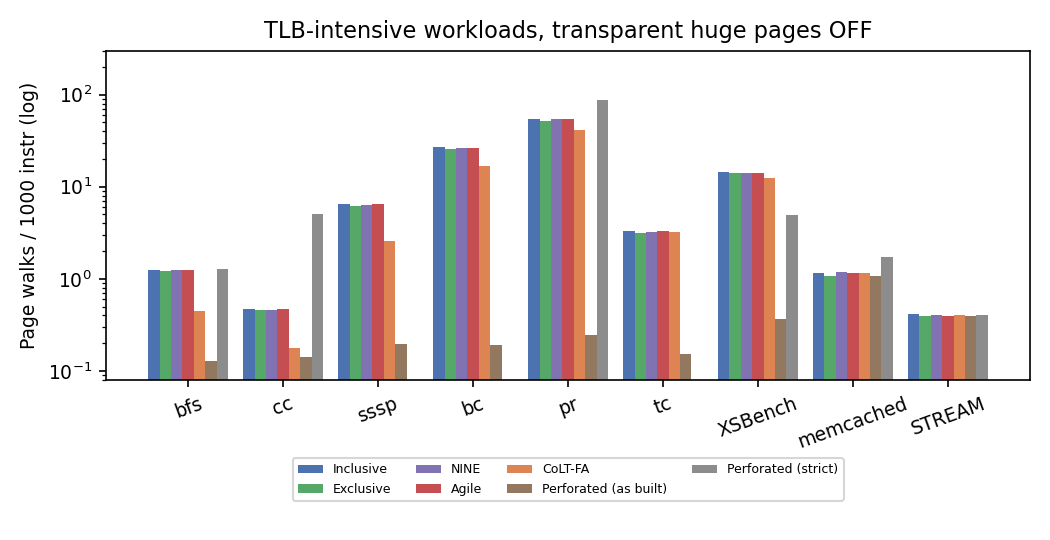
\includegraphics[width=\textwidth]{figures/thp_off_all_designs.png}
\caption{Page walks per 1000 instructions with transparent huge pages off (log scale).}
\label{fig:thpoff_all}
\end{figure}

\begin{table}[htbp]
\centering
\small
\caption{Page walks per 1000 instructions, transparent huge pages off. "Perf." is Perforated Pages as built and "Strict" is the strict variant from Section~\ref{sec:perf_strict}; a dash means not run.}
\label{tab:thpoff_all}
\begin{tabular}{l r r r r r r r}
\toprule
\textbf{Workload} & \textbf{Inclusive} & \textbf{Exclusive} & \textbf{NINE} & \textbf{Agile} & \textbf{CoLT-FA} & \textbf{Perf.} & \textbf{Strict} \\
\midrule
GAPBS bfs & 1.253 & 1.219 & 1.234 & 1.236 & 0.448 & 0.129 & 1.290 \\
GAPBS cc & 0.471 & 0.463 & 0.461 & 0.464 & 0.178 & 0.140 & 5.056 \\
GAPBS sssp & 6.461 & 6.251 & 6.353 & 6.435 & 2.585 & 0.197 & -- \\
GAPBS bc & 26.743 & 25.848 & 26.551 & 26.646 & 16.911 & 0.192 & -- \\
GAPBS pr & 55.046 & 51.821 & 54.760 & 54.692 & 41.812 & 0.244 & 88.556 \\
GAPBS tc & 3.279 & 3.142 & 3.249 & 3.266 & 3.220 & 0.154 & -- \\
XSBench & 14.395 & 13.967 & 14.256 & 14.254 & 12.492 & 0.369 & 4.941 \\
memcached & 1.156 & 1.082 & 1.178 & 1.156 & 1.142 & 1.081 & 1.728 \\
STREAM & 0.414 & 0.399 & 0.400 & 0.399 & 0.400 & 0.399 & 0.400 \\
\bottomrule
\end{tabular}
\end{table}

\noindent Among the inclusion policies, Exclusive gives the fewest walks on every workload (STREAM is a tie), because it does not keep the same translation in both levels and so holds more translations in total (for pr, 51.821 against 55.046 for Inclusive, about 6\% fewer). Inclusive gives the most. The Agile prefetcher gives almost the same numbers as NINE on these workloads. CoLT-FA gives the largest reduction of the realistic designs. Perforated Pages as built shows very low numbers; Section~\ref{sec:perf_strict} explains why these numbers are not realistic.

\subsection{CoLT-FA Compared With NINE}
CoLT-FA is built on NINE, and the same binary runs both. Figure~\ref{fig:colt_vs_nine} shows the change in page walks with huge pages off.

\begin{figure}[htbp]
\centering
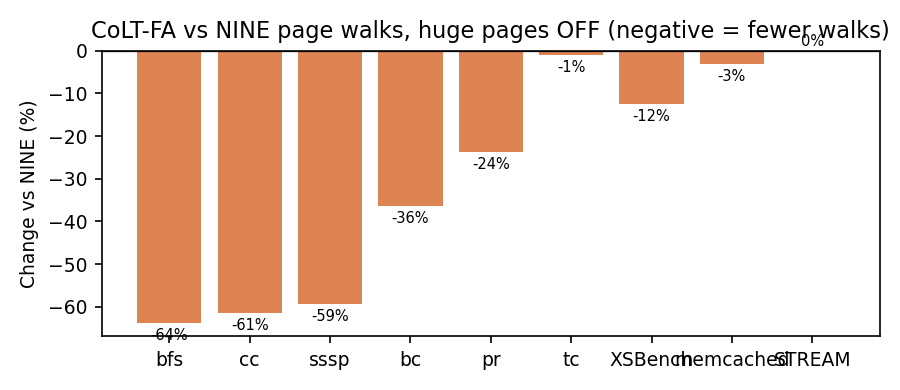
\includegraphics[width=0.85\textwidth]{figures/colt_vs_nine_thpoff.png}
\caption{Change in page walks of CoLT-FA (8 entries) compared with NINE, transparent huge pages off.}
\label{fig:colt_vs_nine}
\end{figure}

\begin{table}[htbp]
\centering
\small
\caption{CoLT-FA (8 entries) against NINE, transparent huge pages off (page walks per 1000 instructions).}
\label{tab:colt_vs_nine}
\begin{tabular}{l r r r}
\toprule
\textbf{Workload} & \textbf{NINE} & \textbf{CoLT-FA} & \textbf{Change} \\
\midrule
GAPBS bfs & 1.234 & 0.448 & $-63.7\%$ \\
GAPBS cc & 0.461 & 0.178 & $-61.4\%$ \\
GAPBS sssp & 6.353 & 2.585 & $-59.3\%$ \\
GAPBS bc & 26.551 & 16.911 & $-36.3\%$ \\
GAPBS pr & 54.760 & 41.812 & $-23.6\%$ \\
XSBench & 14.256 & 12.492 & $-12.4\%$ \\
memcached & 1.178 & 1.142 & $-3.1\%$ \\
GAPBS tc & 3.249 & 3.220 & $-0.9\%$ \\
STREAM & 0.400 & 0.400 & $0.0\%$ \\
\bottomrule
\end{tabular}
\end{table}

\noindent CoLT-FA reduces page walks most on the graph kernels bfs, cc and sssp, by about 59\% to 64\%, and by 36\% and 24\% on bc and pr. These kernels read the graph's large arrays, which the operating system often places on physically contiguous 4KB pages, and that is exactly what CoLT can merge. On XSBench the reduction is 12\%. On memcached, tc and STREAM it is small or zero. For STREAM the buffer received very few hits (57 with 8 entries), which means that in this run the guest did not give STREAM's arrays physically contiguous pages, and CoLT can only merge contiguous pages.

\paragraph{Buffer size.} Figure~\ref{fig:colt_size} compares the default 8-entry buffer with a 32-entry buffer. Going from 8 to 32 entries reduces walks a little further on some workloads (pr from 41.812 to 38.420, bfs from 0.448 to 0.424), but most of the benefit already comes with 8 entries.

\begin{figure}[htbp]
\centering
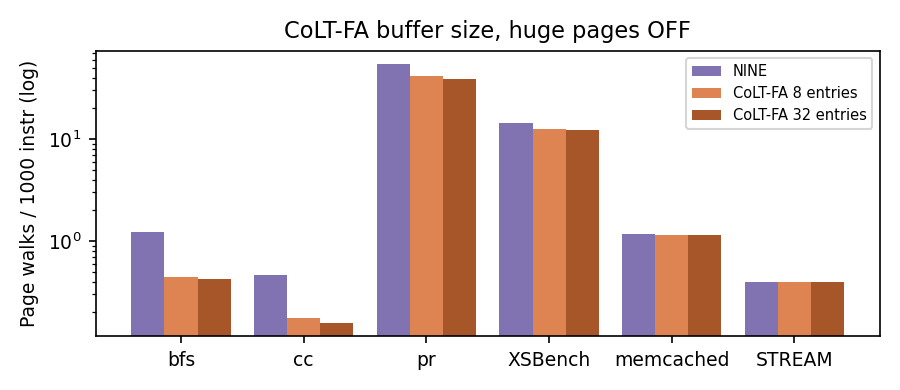
\includegraphics[width=0.85\textwidth]{figures/colt_size.png}
\caption{NINE, CoLT-FA with 8 entries and CoLT-FA with 32 entries, transparent huge pages off.}
\label{fig:colt_size}
\end{figure}

\paragraph{With huge pages on.} Following the same-machine rule, the comparison with huge pages on uses NINE and CoLT-FA runs from the same machine (Table~\ref{tab:colt_thpon} and Figure~\ref{fig:colt_thpon}).

\begin{table}[htbp]
\centering
\small
\caption{CoLT-FA (8 entries) against NINE with transparent huge pages on, each pair from the same machine (page walks per 1000 instructions).}
\label{tab:colt_thpon}
\begin{tabular}{l l r r r}
\toprule
\textbf{Workload} & \textbf{Machine} & \textbf{NINE} & \textbf{CoLT-FA} & \textbf{Change} \\
\midrule
GAPBS bfs & csews36 & 0.118 & 0.062 & $-47.5\%$ \\
GAPBS pr & csews36 & 2.687 & 1.914 & $-28.8\%$ \\
GAPBS bc & csews30 & 6.038 & 4.309 & $-28.6\%$ \\
GAPBS sssp & csews30 & 3.619 & 2.742 & $-24.2\%$ \\
GAPBS cc & csews36 & 0.028 & 0.024 & $-14.3\%$ \\
XSBench & csews36 & 1.138 & 1.102 & $-3.2\%$ \\
STREAM & csews36 & 0.012 & 0.010 & $-16.7\%$ \\
\midrule
519.lbm\_r (ref) & csews24 & 0.375 & 0.076 & $-79.7\%$ \\
523.xalancbmk\_r (ref) & csews24 & 2.608 & 1.453 & $-44.3\%$ \\
520.omnetpp\_r (ref) & csews24 & 2.226 & 1.751 & $-21.3\%$ \\
505.mcf\_r (ref) & csews24 & 3.655 & 3.614 & $-1.1\%$ \\
\bottomrule
\end{tabular}
\end{table}

\noindent With huge pages on, CoLT-FA still reduces page walks, by 47.5\% on bfs and by about 24\% to 29\% on pr, bc and sssp. The absolute numbers are much smaller than with huge pages off, so the remaining walks come from memory that is still mapped with 4KB pages, which is the part CoLT-FA can coalesce. On cc and STREAM the values are very small (below 0.03), so their percentages rest on few walks. The four SPEC reference benchmarks in the lower part of the table were also run on one machine with the same binary. CoLT-FA reduces walks by 79.7\% on lbm, 44.3\% on xalancbmk and 21.3\% on omnetpp, while mcf is almost unchanged ($-1.1\%$).

\begin{figure}[htbp]
\centering
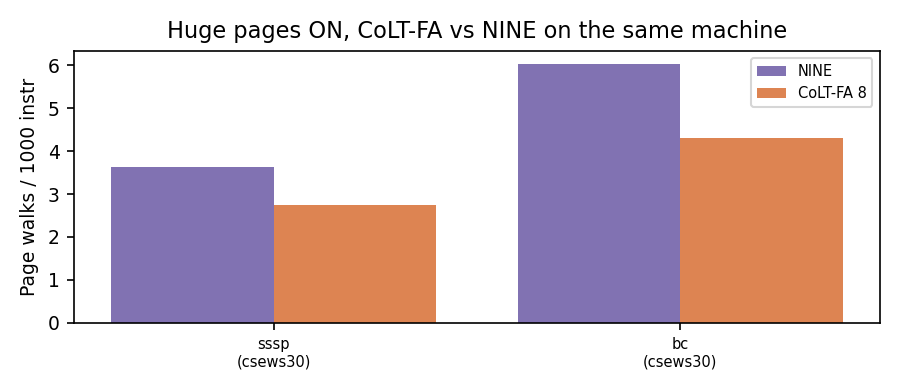
\includegraphics[width=0.75\textwidth]{figures/colt_vs_nine_thpon_samehost.png}
\caption{CoLT-FA against NINE with transparent huge pages on, both runs on the same machine.}
\label{fig:colt_thpon}
\end{figure}

\subsection{The Effect of Huge Pages}
Figure~\ref{fig:thp_effect} shows NINE with transparent huge pages off and on, from the same binary on the same machine. Huge pages remove most of the page walks: pr goes from 54.760 to 2.687, XSBench from 14.256 to 1.138, and bfs from 1.234 to 0.118. memcached barely changes (1.178 to 1.117). This shows that, when the operating system can give a program 2MB pages, much of the TLB pressure disappears, and the designs then differ less. CoLT-FA is most useful in the opposite case, when memory ends up in 4KB pages.

\begin{figure}[htbp]
\centering
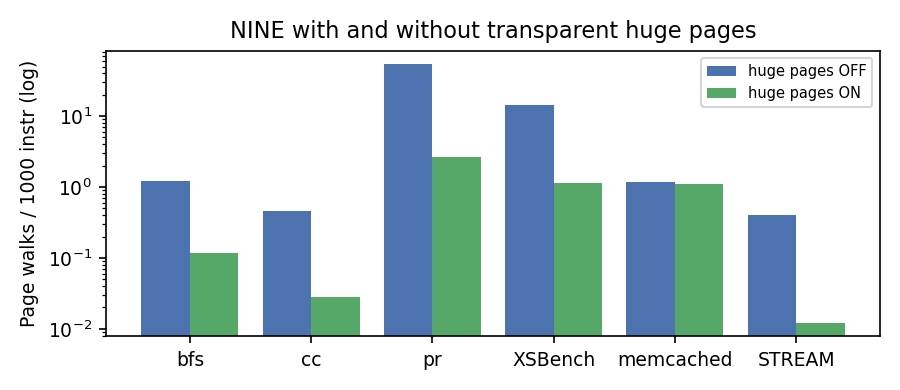
\includegraphics[width=0.85\textwidth]{figures/thp_effect_nine.png}
\caption{NINE with transparent huge pages off and on (same binary, same machine).}
\label{fig:thp_effect}
\end{figure}

\subsection{SPEC CPU2017 Reference Inputs}
Nine SPEC benchmarks were run with reference inputs, measured for 200M instructions after 3G instructions of warm-up, with huge pages on. Each design ran on its own machine, so following the rule above these numbers are reported per design and are not used for small differences. Table~\ref{tab:ref} shows the results for the four inclusion and prefetching designs, which agree with each other closely. With real input sizes mcf (3.360 to 3.695) and omnetpp (2.172 to 2.324) are the most TLB-intensive, far above their test-input values.

\begin{table}[htbp]
\centering
\small
\caption{SPEC CPU2017 reference inputs, page walks per 1000 instructions (huge pages on, each design on its own machine).}
\label{tab:ref}
\begin{tabular}{l r r r r}
\toprule
\textbf{Benchmark} & \textbf{Inclusive} & \textbf{Exclusive} & \textbf{NINE} & \textbf{Agile} \\
\midrule
505.mcf\_r & 3.695 & 3.360 & 3.617 & 3.613 \\
523.xalancbmk\_r & 2.625 & 2.623 & 2.609 & 2.614 \\
520.omnetpp\_r & 2.324 & 2.172 & 2.232 & 2.267 \\
503.bwaves\_r & 0.486 & 0.476 & 0.481 & 0.483 \\
519.lbm\_r & 0.378 & 0.369 & 0.374 & 0.375 \\
554.roms\_r & 0.346 & 0.333 & 0.340 & 0.344 \\
531.deepsjeng\_r & 0.171 & 0.161 & 0.164 & 0.165 \\
557.xz\_r & 0.132 & 0.128 & 0.129 & 0.133 \\
\bottomrule
\end{tabular}
\end{table}

\noindent 549.fotonik3d\_r gave no window on any design: its first program finished before the 3G-instruction warm-up ended.

% -----------------------------------------------------------------------------
\section{A Second Look at Perforated Pages}
\label{sec:perf_strict}
% -----------------------------------------------------------------------------

In Table~\ref{tab:thpoff_all}, Perforated Pages as built shows close to zero page walks on almost every workload, far fewer than any other design. While looking into this we found the reason in the model itself. Each L2 entry covers a 2MB virtual region, but it stores a \emph{separate physical address for each of its 512 4KB pages} (\texttt{paddrs[512]}), and it never checks that these pages are physically contiguous. With 128 sets of 4 ways, the L2 can therefore hold up to $128 \times 4 \times 512 = 262{,}144$ unrelated 4KB translations, about 512 times the reach of the other designs' 512-entry L2. Real perforated pages are 2MB regions that are physically contiguous apart from their holes, so one base address and a bitmap are enough to describe them.

To measure the design under the paper's rule, we added a strict mode (\texttt{PERF\_STRICT=1}, produced by \texttt{robustness/patches/make\_perf\_strict.py}). A 4KB page may join a region only if its physical address equals the region's base address plus its offset. Otherwise the region is started again from the new page. The default behaviour is unchanged, so the earlier results stay reproducible.

\begin{table}[htbp]
\centering
\small
\caption{Perforated Pages as built and in strict mode, compared with NINE (page walks per 1000 instructions).}
\label{tab:perf_strict}
\begin{tabular}{l l r r r}
\toprule
\textbf{Workload} & \textbf{Huge pages} & \textbf{NINE} & \textbf{As built} & \textbf{Strict} \\
\midrule
GAPBS bfs & off & 1.234 & 0.129 & 1.290 \\
GAPBS cc & off & 0.461 & 0.140 & 5.056 \\
GAPBS pr & off & 54.760 & 0.244 & 88.556 \\
XSBench & off & 14.256 & 0.369 & 4.941 \\
memcached & off & 1.178 & 1.081 & 1.728 \\
505.mcf\_r (ref) & on & 3.617 & 0.124 & 10.352 \\
520.omnetpp\_r (ref) & on & 2.232 & 0.567 & 9.058 \\
523.xalancbmk\_r (ref) & on & 2.609 & 0.185 & 4.899 \\
\bottomrule
\end{tabular}
\end{table}

\noindent With the strict rule, Perforated Pages has \emph{more} page walks than NINE on most workloads (for example pr 88.556 against 54.760, and mcf 10.352 against 3.617). Every entry is tied to a 2MB virtual region, so memory made of scattered 4KB pages wastes most of each entry, and regions are restarted often. XSBench is the exception (4.941 against 14.256). We conclude that the large gains measured for Perforated Pages in this project, including those in Section~6 of Part~\ref{part:mid}, come mostly from the unlimited per-page storage of the model and not from the perforated-page idea. A fair evaluation of Perforated Pages would also need the operating system support from the paper, which creates the sparse 2MB regions in the first place. For these reasons we treat CoLT-FA as the main realistic design of this project.

% -----------------------------------------------------------------------------
\section{Limitations and Notes on Method}
\label{sec:limits}
% -----------------------------------------------------------------------------
\begin{itemize}
    \item \textbf{Memory limit.} The \texttt{X86Board} allows at most 3 GiB of guest memory, so 631.deepsjeng\_s and 619.lbm\_s were checked in SE mode only (both PASS on all designs).
    \item \textbf{x87 emulation.} The perlbench failures are caused by \texttt{gem5}, not by the TLB designs, and affect every design.
    \item \textbf{Sampled windows.} Performance numbers come from windows of 200M to 1.5G instructions, not from whole runs. Correctness is still checked over the whole run for SPEC test inputs.
    \item \textbf{Same-machine rule.} With transparent huge pages on, the guest's memory layout depends on the disk image built on each machine, so these results are only compared within one machine.
    \item \textbf{Single core.} All full-system runs use one simulated core.
    \item \textbf{Redis.} Redis was also prepared as a second key-value store. The first runs stopped making progress inside the guest before the measured phase and were stopped after two days. A second attempt with time limits and progress messages on every step was started on the last day. memcached covers the key-value store case in this report.
    \item \textbf{The Hybrid L2 TLB} from Part~\ref{part:mid} was not part of the second phase.
\end{itemize}

% -----------------------------------------------------------------------------
\section{Conclusion}
% -----------------------------------------------------------------------------
In the first half of the project we built set-associative L2 TLB designs with different inclusion policies, prefetching, CoLT-FA, Perforated Pages and a Hybrid in \texttt{gem5}, and measured them in SE mode on microbenchmarks. In the second half we audited all of them and fixed the problems that only show up under a real operating system: missing L2 invalidation on unmaps and address-space switches, PCID handling, checkpointing, and hard-coded permissions. We added a translation oracle and invariant checkers and found no translation error in any design. We rebuilt CoLT-FA so that it coalesces pages from the hardware page walker, as in the original paper, which made it work in full-system mode for the first time.

In full-system mode on an Ubuntu guest, every SPEC CPU2017 benchmark that the simulator can run passed on all six designs. The only failures came from a \texttt{gem5} floating-point emulation bug and from the 3 GiB memory limit, and the two large benchmarks passed in SE mode with more memory. On the graph and key-value workloads, CoLT-FA reduced page walks compared with NINE by 59\% to 64\% on bfs, cc and sssp, by 36\% on bc and by 24\% on pr with 4KB pages, and, on the same machine with huge pages on, by 47.5\% on bfs and by about 24\% to 29\% on pr, bc and sssp. On SPEC reference inputs it reduced walks by 79.7\% on lbm, 44.3\% on xalancbmk and 21.3\% on omnetpp. Exclusive was the best of the inclusion policies. A closer look at Perforated Pages showed that its large gains came from an unrealistic model, and under the paper's rule it did worse than NINE on most workloads.


\newpage
\begin{appendices}
% =============================================================================
% APPENDIX A: ARTIFACT DESCRIPTION AND EVALUATION INSTRUCTIONS
% =============================================================================
\section{Artifact Description and Evaluation Instructions}
\label{app:artifact}

The submitted folder contains this report, \texttt{declaration.txt}, a \texttt{README.md} with the same content as this appendix in more detail, the LaTeX source of the report, and the \texttt{artifact/} directory described below.

\subsection{Directory Structure}
\begin{table}[H]
\centering
\small
\begin{tabularx}{\textwidth}{l X}
\toprule
\textbf{Path} & \textbf{Contents} \\
\midrule
\texttt{artifact/gem5\_patches/} & \texttt{tlb.\{cc,hh\}.<d>.fixed} for $d \in$ \{inc, excl, nine, agile, perf, colt\}, \texttt{tlb.\{cc,hh\}.perf.strict}, \texttt{pagetable\_walker.cc.colt}, the generators \texttt{make\_colt\_fixed.py} and \texttt{make\_perf\_strict.py}, the checker scripts \texttt{apply\_checker*.py}, diffs against the mid-review snapshots, and \texttt{midreview/} with the mid-review snapshots. \\
\texttt{artifact/benchmarks/} & \texttt{tests/} (tlbstress, pf\_patterns, perf\_holes, gups), \texttt{microbench/} (mid-review microbenchmarks), \texttt{stdbench/} (memcached and Redis drivers), \texttt{spec/} (SPEC CPU2017 build configuration). \\
\texttt{artifact/configs/} & \texttt{fs\_run.py}, the full-system configuration. \\
\texttt{artifact/scripts/} & Build, run, collect and plot automation (Table~\ref{tab:art_scripts}). \\
\texttt{artifact/results/} & \texttt{windows.csv} (554 timing windows), \texttt{spec\_fs\_matrix.csv} (238 SPEC verdicts), \texttt{se\_bigmem.csv}, \texttt{colt\_se\_verification.csv}, \texttt{figures/} with \texttt{numbers.txt}, and \texttt{design\_reports/} (audit and SE reports of each design). \\
\bottomrule
\end{tabularx}
\end{table}

\begin{table}[H]
\centering
\small
\caption{Main scripts.}
\label{tab:art_scripts}
\begin{tabularx}{\textwidth}{l X}
\toprule
\textbf{Script} & \textbf{Role} \\
\midrule
\texttt{build\_design.sh <gem5> <d> [--checker]} & Copies the design's files into a gem5 25.1.0.1 tree (and the walker for CoLT-FA), optionally adds the checker, and builds \texttt{gem5.opt}. \\
\texttt{quick\_start.sh <gem5>} & Five-minute SE check of CoLT-FA with the oracle, with the buffer on and off. Also runs the user's own program. \\
\texttt{build\_microbench.sh}, \texttt{build\_stdbench.sh} & Build the test programs and download and build GAPBS, XSBench, STREAM, memcached, mc-crusher and Redis as static binaries. \\
\texttt{run\_spec\_fs\_shards.sh} & Full-system SPEC CPU2017 runs, one \texttt{gem5} per benchmark, with measurement windows. \\
\texttt{run\_stdbench\_fs3.sh}, \texttt{run\_micro\_fs.sh} & Full-system runs of the standard workloads and microbenchmarks. \\
\texttt{se\_bigmem.sh} & SE runs with 8 GiB and byte-by-byte output comparison. \\
\texttt{gen\_se\_jobs.py}, \texttt{runner.py} & SE correctness job matrix and parallel runner. \\
\texttt{provision\_fs\_host.sh}, \texttt{sync\_fs\_results.sh} & Copy a design's inputs to a new machine; copy results back. \\
\texttt{collect\_results.py}, \texttt{plot\_results.py} & Turn all output into CSV tables and draw every figure of Part~\ref{part:post}. \\
\bottomrule
\end{tabularx}
\end{table}

\subsection{Features and Test Scenarios}
\begin{table}[H]
\centering
\small
\begin{tabularx}{\textwidth}{l X X X}
\toprule
\textbf{Feature} & \textbf{Test scenario} & \textbf{Script} & \textbf{Expected outcome} \\
\midrule
L2 invalidation on unmap and CR3 switch & FS SPEC CPU2017; SE \texttt{tlbstress remap} & \texttt{run\_spec\_fs\_shards.sh}, \texttt{runner.py} & SPEC output check passes; 0 oracle mismatches \\
PCID-aware L2 & SE multi-process jobs; FS runs & \texttt{gen\_se\_jobs.py} & 0 oracle mismatches \\
Runtime parameters & \texttt{NINE\_L2\_SETS}, \texttt{EXCL\_SPILL}, \texttt{AGILE\_PF\_*}, \texttt{COLT\_FA\_ENTRIES}, \texttt{PERF\_STRICT} & any run & statistics change, correctness unchanged \\
Translation oracle and checkers & \texttt{TLBCHK\_FS\_PERIOD}, \texttt{TLBCHK\_MAXWARN}, \texttt{TLBCHK\_PANIC} & \texttt{build\_design.sh --checker} & \texttt{chkOracleMismatch} = 0 \\
CoLT-FA in full system & \texttt{COLT\_ENABLE=1/0}, 8 or 32 entries, huge pages on/off & \texttt{run\_stdbench\_fs3.sh}, \texttt{quick\_start.sh} & CoLT hits only when enabled; fewer walks on graph workloads \\
Measurement windows & \texttt{WINDOW\_WARM}, \texttt{WINDOW\_INSTS}, \texttt{WINDOW\_EXIT} & \texttt{run\_spec\_fs\_shards.sh} & one statistics dump per benchmark \\
\bottomrule
\end{tabularx}
\end{table}

\noindent \textbf{Findings while running the tests.} perlbench fails on every design in full-system mode (gem5 x87 emulation bug); 631.deepsjeng\_s fails in full-system mode (memory limit) and passes in SE mode; 619.lbm\_s triggers the \texttt{gem5} assertion \texttt{Packet::setCacheResponding(): !flags.isSet(CACHE\_RESPONDING)} on every design right after its window, and passes in SE mode; the first Redis runs made no progress inside the guest. The SE-mode failures (\texttt{setitimer}, fork with shared memory, multi-process remap) are identical on stock \texttt{gem5}.

\subsection{Assumptions and Unsupported Features}
\texttt{gem5} 25.1.0.1 for x86, gcc-11, Python 3.10 and scons 4.8.1. Full-system runs need the \texttt{gem5} resources kernel \texttt{vmlinux-x86-ubuntu-6.8.0-52-generic} and disk image \texttt{x86-ubuntu-24.04.img}, and a licensed SPEC CPU2017 installation (not included). Single simulated core and at most 3 GiB guest memory. Without KVM the guest boots on the atomic CPU. The Hybrid L2 TLB is included only as a mid-review snapshot.

\subsection{Getting Started (about 30 minutes with a built tree)}
\begin{table}[H]
\centering
\small
\begin{tabularx}{\textwidth}{l X l l}
\toprule
\textbf{Step} & \textbf{Command} & \textbf{Human} & \textbf{Compute} \\
\midrule
1 & \texttt{git clone https://github.com/gem5/gem5 -b v25.1.0.1} & 2 min & 5 min \\
2 & \texttt{bash artifact/scripts/build\_design.sh <gem5> colt --checker -j 16} & 1 min & 1--2 h clean, 6 min on a built tree \\
3 & \texttt{bash artifact/scripts/quick\_start.sh <gem5>} & 1 min & under 1 min \\
4 & \texttt{python3 artifact/scripts/plot\_results.py artifact/results /tmp/fig} & 1 min & 10 s \\
\bottomrule
\end{tabularx}
\end{table}

\noindent In our test on a stock \texttt{gem5} 25.1.0.1 tree, step 2 took 6 minutes and step 3 took under a minute. For the ascending pattern it reported 14,330 CoLT hits and 10,329 walks with CoLT on, against 24,659 walks with CoLT off. Step 3 should print \texttt{oracleMismatch=0} on every line, and CoLT hits above zero with fewer walks when CoLT is enabled. To use one's own program: \texttt{QS\_PROG=/path/to/static\_binary QS\_ARGS="..." bash artifact/scripts/quick\_start.sh <gem5>}.

\subsection{Detailed Evaluation}
\begin{table}[H]
\centering
\small
\begin{tabularx}{\textwidth}{l X X l X}
\toprule
\textbf{\#} & \textbf{Experiment and purpose} & \textbf{How to run} & \textbf{Runtime} & \textbf{Expected result and location} \\
\midrule
E1 & SE correctness matrix of a design against stock \texttt{gem5} & \texttt{gen\_se\_jobs.py}, then \texttt{runner.py <jobs> --jobs 24} & 3--6 h & 0 mismatches; Table~\ref{tab:se_matrix}; \texttt{design\_reports/} \\
E2 & CoLT-FA SE checks, buffer on/off & \texttt{quick\_start.sh} or the 36-run loop & 10 min & 36/36 PASS; Table~\ref{tab:colt_se}; \texttt{colt\_se\_verification.csv} \\
E3 & SPEC CPU2017 full system, test inputs & \texttt{run\_spec\_fs\_shards.sh <d> 43 atomic} with \texttt{WINDOW\_INSTS=200000000 WINDOW\_WARM=50000000} & 1--3 days & 37/43 PASS; Table~\ref{tab:spec_outcome}; \texttt{spec\_fs\_matrix.csv} \\
E4 & SE 8 GiB runs of deepsjeng\_s and lbm\_s & \texttt{se\_bigmem.sh <bench> inc excl nine agile perf colt} & 6--16 h & PASS on all; Table~\ref{tab:se_bigmem}; \texttt{se\_bigmem.csv} \\
E5 & TLB-intensive workloads per design, huge pages on/off & \texttt{build\_stdbench.sh}; \texttt{[THP=never] [COLT\_ENABLE=0] STD\_TAG=<t> run\_stdbench\_fs3.sh <d>} & 4--7 h & Tables~\ref{tab:thpoff_all} and~\ref{tab:colt_vs_nine}; \texttt{windows.csv} \\
E6 & SPEC reference windows & \texttt{SPEC\_FS\_SIZE=ref WINDOW\_WARM=3000000000 WINDOW\_EXIT=1 run\_spec\_fs\_shards.sh <d> 9 atomic <benches>} & about 5 h & Table~\ref{tab:ref}; \texttt{windows.csv} \\
E7 & Perforated Pages strict mode & build \texttt{perfstrict}, run E5/E6 with \texttt{PERF\_STRICT=1} & as E5/E6 & Table~\ref{tab:perf_strict} \\
E8 & Tables and plots & \texttt{collect\_results.py <mirror> out}; \texttt{plot\_results.py out out/figures} & 1 min & all figures of Part~\ref{part:post} \\
\bottomrule
\end{tabularx}
\end{table}

\end{appendices}

% -----------------------------------------------------------------------------
\begin{thebibliography}{99}

\bibitem{binkert2011gem5}
N.~Binkert, B.~Beckmann, G.~Black, S.~K. Reinhardt, A.~Saidi, A.~Basu, J.~Hestness, D.~R. Hower, T.~Krishna, S.~Sardashti, et~al.,
\newblock ``The gem5 simulator,''
\newblock \textit{ACM SIGARCH Computer Architecture News}, vol.~39, no.~2, pp.~1--7, 2011.

\bibitem{seznec1993skewed}
A.~Seznec,
\newblock ``A case for two-way skewed-associative caches,''
\newblock in \textit{Proceedings of the 20th Annual International Symposium on Computer Architecture (ISCA)}, pp.~169--178, 1993.

\bibitem{baer1988multi}
J.-L. Baer and W.-H. Wang,
\newblock ``On the inclusion properties for multi-level cache hierarchies,''
\newblock in \textit{Proceedings of the 15th Annual International Symposium on Computer Architecture (ISCA)}, pp.~73--80, 1988.

\bibitem{margaritov2019prefetched}
A.~Margaritov, D.~Ustiugov, E.~Bugnion, and B.~Grot,
\newblock ``Prefetched address translation,''
\newblock in \textit{Proceedings of the 52nd Annual IEEE/ACM International Symposium on Microarchitecture (MICRO)}, pp.~1013--1026, 2019.

\bibitem{vavouliotis2021agile}
G.~Vavouliotis, L.~Alvarez, V.~Karakostas, K.~Nikas, N.~Koziris, D.~A. Jim\'enez, and M.~Casas,
\newblock ``Exploiting page table locality for agile TLB prefetching,''
\newblock in \textit{Proceedings of the 48th Annual International Symposium on Computer Architecture (ISCA)}, 2021.

\bibitem{pham2012colt}
B.~Pham, V.~Vaidyanathan, A.~Jaleel, and A.~Bhattacharjee,
\newblock ``CoLT: Coalesced Large-Reach TLBs,''
\newblock in \textit{Proceedings of the 45th Annual IEEE/ACM International Symposium on Microarchitecture (MICRO)}, pp.~258--269, 2012.

\bibitem{kwon2020perforated}
C.~H. Park, S.~Cha, B.~Kim, Y.~Kwon, D.~Black-Schaffer, and J.~Huh,
\newblock ``Perforated Page: Supporting fragmented memory allocation for large pages,''
\newblock in \textit{Proceedings of the 47th ACM/IEEE Annual International Symposium on Computer Architecture (ISCA)}, 2020.

\bibitem{beamer2015gap}
S.~Beamer, K.~Asanovi\'c, and D.~Patterson,
\newblock ``The GAP benchmark suite,''
\newblock \textit{arXiv:1508.03619}, 2015.

\bibitem{tramm2014xsbench}
J.~R. Tramm, A.~R. Siegel, T.~Islam, and M.~Schulz,
\newblock ``XSBench: the development and verification of a performance abstraction for Monte Carlo reactor analysis,''
\newblock in \textit{PHYSOR 2014: The Role of Reactor Physics toward a Sustainable Future}, 2014.

\bibitem{mccalpin1995stream}
J.~D. McCalpin,
\newblock ``Memory bandwidth and machine balance in current high performance computers,''
\newblock \textit{IEEE Computer Society Technical Committee on Computer Architecture (TCCA) Newsletter}, pp.~19--25, 1995.

\bibitem{memcached}
memcached, a distributed memory object caching system, \url{https://memcached.org}; load generator \texttt{mc-crusher}, \url{https://github.com/memcached/mc-crusher}.

\bibitem{spec2017}
Standard Performance Evaluation Corporation, ``SPEC CPU2017,'' \url{https://www.spec.org/cpu2017/}.

\bibitem{yan2024trail}
Z.~Yan, J.~Zhao, Y.~Zhang, and M.~Zhang,
\newblock ``Trail: Scalable temporal address translation by embedding deltas in page tables,''
\newblock in \textit{Proceedings of the 29th ACM International Conference on Architectural Support for Programming Languages and Operating Systems (ASPLOS)}, pp.~412--426, 2024.

\bibitem{song2023revelator}
J.~Song, S.~Woo, H.~Park, and Y.~Kim,
\newblock ``Revelator: Rapid speculative translation using XOR inversion for high-performance processors,''
\newblock in \textit{Proceedings of the 50th Annual International Symposium on Computer Architecture (ISCA)}, pp.~1--14, 2023.

\bibitem{skarlatos2023snakebyte}
D.~Skarlatos, Q.~Zhang, E.~Bugg, and C.~Fletcher,
\newblock ``SnakeByte: Adaptive and recursive page merging for virtual memory,''
\newblock in \textit{Proceedings of the 29th IEEE International Symposium on High-Performance Computer Architecture (HPCA)}, pp.~589--602, 2023.

\bibitem{kim2024star}
D.~Kim, M.~Park, S.~Lee, and K.~Kang,
\newblock ``STAR: Sub-entry sharing-aware TLB for multi-tenant and virtualized systems,''
\newblock in \textit{Proceedings of the 57th IEEE/ACM International Symposium on Microarchitecture (MICRO)}, pp.~784--797, 2024.

\bibitem{marching2025hpca}
H.~Lin, C.~Peng, T.~Mao, and K.~Wang,
\newblock ``Marching page walks: Hardware concurrency for massive translation outliers,''
\newblock in \textit{Proceedings of the 31st IEEE International Symposium on High-Performance Computer Architecture (HPCA)}, 2025.

\end{thebibliography}

\end{document}
